\chapter{HASIL DAN PEMBAHASAN}
\label{chap:hasil_dan_pembahasan}

Bab ini membahas hasil pengujian sistem PWM AC \emph{chopper} yang telah
dirancang. Pengujian dilakukan untuk mengetahui karakteristik sinyal PWM,
hubungan \emph{duty cycle} terhadap tegangan RMS keluaran, respons tekanan
air pada pompa, serta kelayakan data yang digunakan untuk pelatihan algoritma
\emph{neural network}.

\section{Skenario Pengujian}
\label{sec:skenario-pengujian}

Pengujian dilakukan secara bertahap dari tingkat komponen hingga sistem
terintegrasi, sesuai Tabel~\ref{tab:skenario-pengujian}.

\begin{table}[H]
\centering
\caption{Skenario pengujian sistem}
\label{tab:skenario-pengujian}
\begin{tabularx}{\linewidth}{|c|>{\raggedright\arraybackslash\hsize=0.9\hsize}X|>{\raggedright\arraybackslash\hsize=1.1\hsize}X|}
\hline
\textbf{No.} &
\textbf{Pengujian} &
\textbf{Tujuan} \\
\hline
1 & Sinyal PWM STM32 &
Memvalidasi frekuensi, \emph{duty cycle}, dan sinyal komplementer \\
\hline
2 & PWM AC \emph{chopper} tanpa beban &
Mengetahui hubungan \emph{duty cycle} terhadap tegangan RMS \\
\hline
3 & PWM AC \emph{chopper} dengan beban pompa &
Mengukur tegangan RMS, arus, dan tekanan aktual \\
\hline
4 & Sensor tekanan air &
Memverifikasi akurasi ADC terhadap tekanan referensi \\
\hline
5 & Dataset \emph{neural network} &
Mengakuisisi data latih dan data uji dengan variasi beban \\
\hline
6 & Model \emph{neural network} &
Mengevaluasi RMSE, MAE, dan R$^2$ prediksi \emph{duty cycle} \\
\hline
\end{tabularx}
\end{table}

\section{Pengujian Sinyal PWM STM32}
\label{sec:pengujian-pwm-stm32}

Pengujian sinyal PWM dilakukan untuk memastikan bahwa mikrokontroler STM32
menghasilkan dua sinyal kendali sesuai kebutuhan rangkaian PWM AC
\emph{chopper}. Sinyal utama diamati pada pin PA8, sedangkan sinyal
komplementer diamati pada pin PA7. Parameter yang diamati meliputi frekuensi,
\emph{duty cycle}, beda fasa sinyal, dan keberadaan \emph{dead time}. Bentuk
sinyal PWM STM32 pada dua nilai \emph{duty cycle} ditunjukkan pada
Gambar~\ref{fig:pwm-stm32}, sedangkan hasil pengukuran \emph{duty cycle} sinyal
aktif (PA8) dan sinyal \emph{freewheeling} (PA7) pada rentang 10--95\%
dirangkum pada Tabel~\ref{tab:hasil-pwm-stm32}. Frekuensi PWM dijaga konstan
pada 5,05~kHz (target 5~kHz). Hasil pengujian sinyal PWM STM32 pada osiloskop
ditunjukkan pada Gambar~\ref{fig:uji-pwm-stm}.

\begin{figure}[H]
  \centering
  \begin{subfigure}{0.49\textwidth}
    \centering
    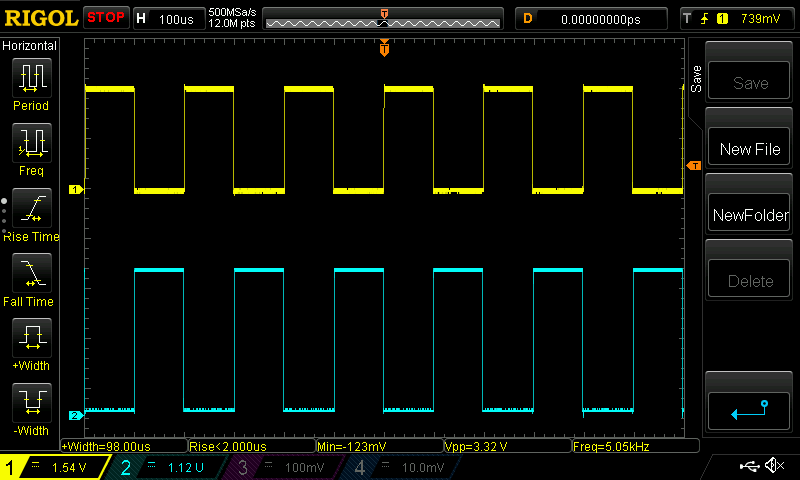
\includegraphics[width=\textwidth]{gambar/pwm_stm32_dc50}
    \caption{\emph{Duty cycle} 50\%}
    \label{fig:pwm-stm32-dc50}
  \end{subfigure}\hfill
  \begin{subfigure}{0.49\textwidth}
    \centering
    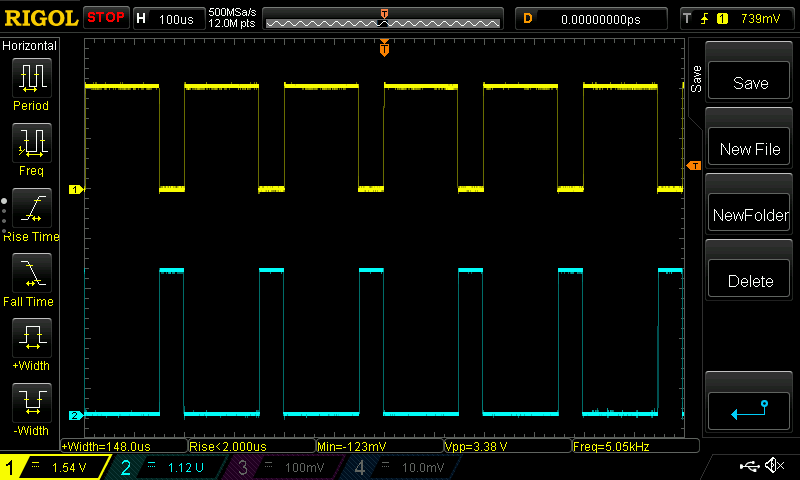
\includegraphics[width=\textwidth]{gambar/pwm_smt32_dc75}
    \caption{\emph{Duty cycle} 75\%}
    \label{fig:pwm-stm32-dc75}
  \end{subfigure}
  \caption{Sinyal PWM STM32 (kuning: PA8 utama; biru: PA7 komplementer)}
  \label{fig:pwm-stm32}
\end{figure}

\begin{figure}[H]
  \centering
  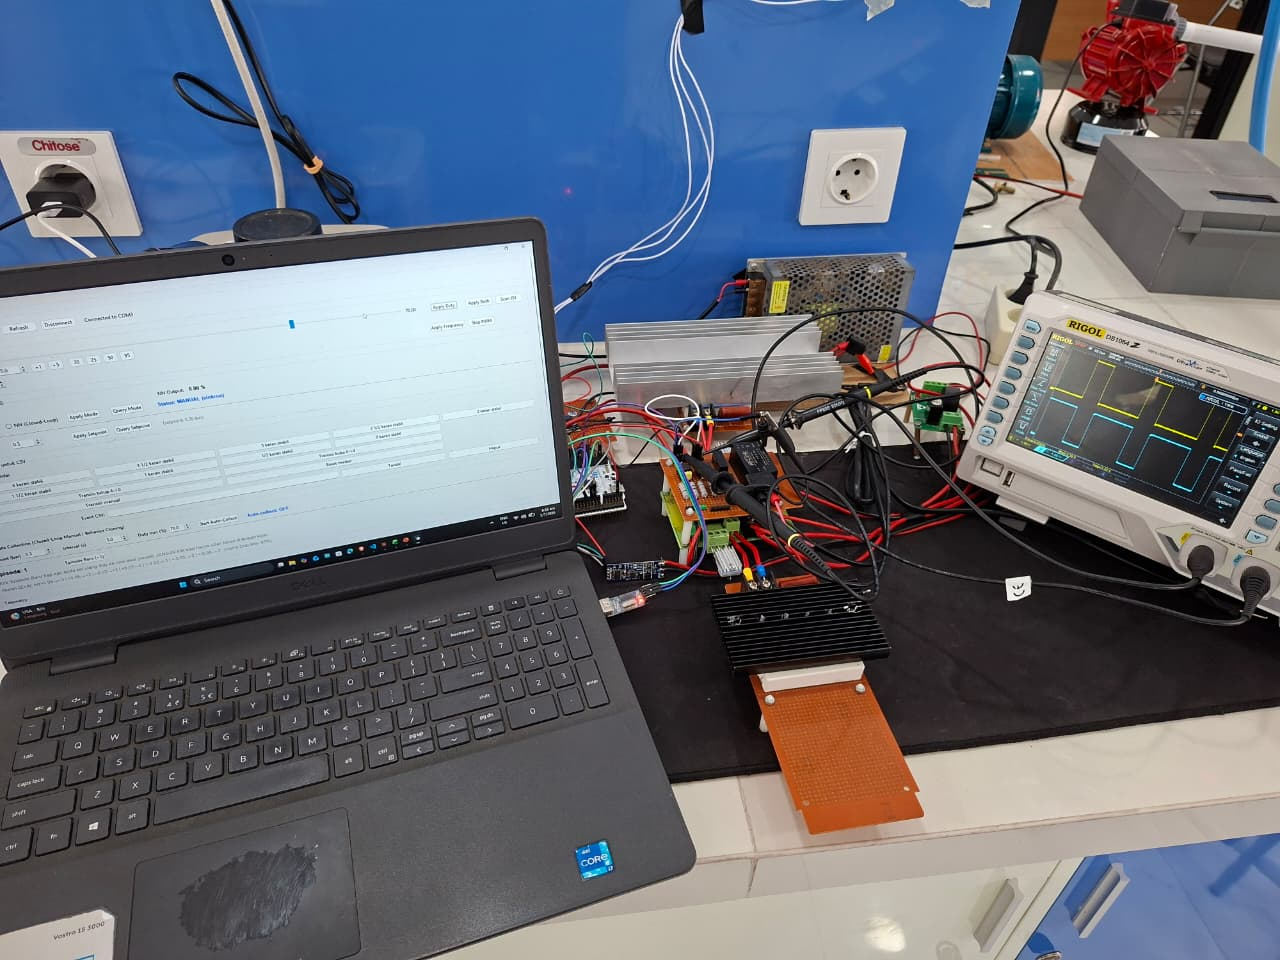
\includegraphics[width=0.55\textwidth]{gambar/uji_pwm_stm}
  \caption{Dokumentasi pengujian sinyal PWM STM32}
  \label{fig:uji-pwm-stm}
\end{figure}

\begin{table}[H]
\centering
\caption{Hasil pengujian \emph{duty cycle} sinyal PWM STM32 (PA8 dan PA7)}
\label{tab:hasil-pwm-stm32}
  \begin{tabularx}{\linewidth}{|c|>{\centering\arraybackslash}X|>{\centering\arraybackslash}X|>{\centering\arraybackslash}X|}
\hline
\textbf{No.} &
\textbf{\emph{Duty Cycle} Diatur (\%)} &
\textbf{\emph{Duty Cycle} Aktif PA8 (\%)} &
\textbf{\emph{Duty Cycle} \emph{Freewheeling} PA7 (\%)} \\
\hline
1 & 10 & 9,05 & 89,90 \\
\hline
2 & 20 & 19,09 & 79,80 \\
\hline
3 & 30 & 29,14 & 69,70 \\
\hline
4 & 40 & 39,19 & 59,59 \\
\hline
5 & 50 & 49,25 & 49,49 \\
\hline
6 & 60 & 59,00 & 39,39 \\
\hline
7 & 70 & 69,00 & 29,29 \\
\hline
8 & 80 & 78,89 & 19,19 \\
\hline
9 & 90 & 89,94 & 9,09 \\
\hline
10 & 95 & 93,97 & 4,04 \\
\hline
\end{tabularx}
\end{table}

\emph{Dead time} antara kedua sinyal komplementer diukur menggunakan kursor
osiloskop pada saat transisi, sebagaimana ditunjukkan pada
Gambar~\ref{fig:dead-time}. Hasil pengukuran pada kedua tepi transisi
masing-masing sebesar 1,48~$\mu$s dan 1,49~$\mu$s, sangat dekat dengan nilai
rancangan 1,5~$\mu$s (Subbab~\ref{sec:penentuan-dead-time}). Dengan adanya
\emph{dead time} ini, tidak terjadi kondisi kedua IGBT satu kaki menghantar
bersamaan (\emph{shoot-through}).
Hasil pengujian sinyal PWM komplementer ditunjukkan pada Tabel~\ref{tab:pwm-komplementer}.

\begin{figure}[htbp]
  \centering
  \begin{subfigure}{0.49\textwidth}
    \centering
    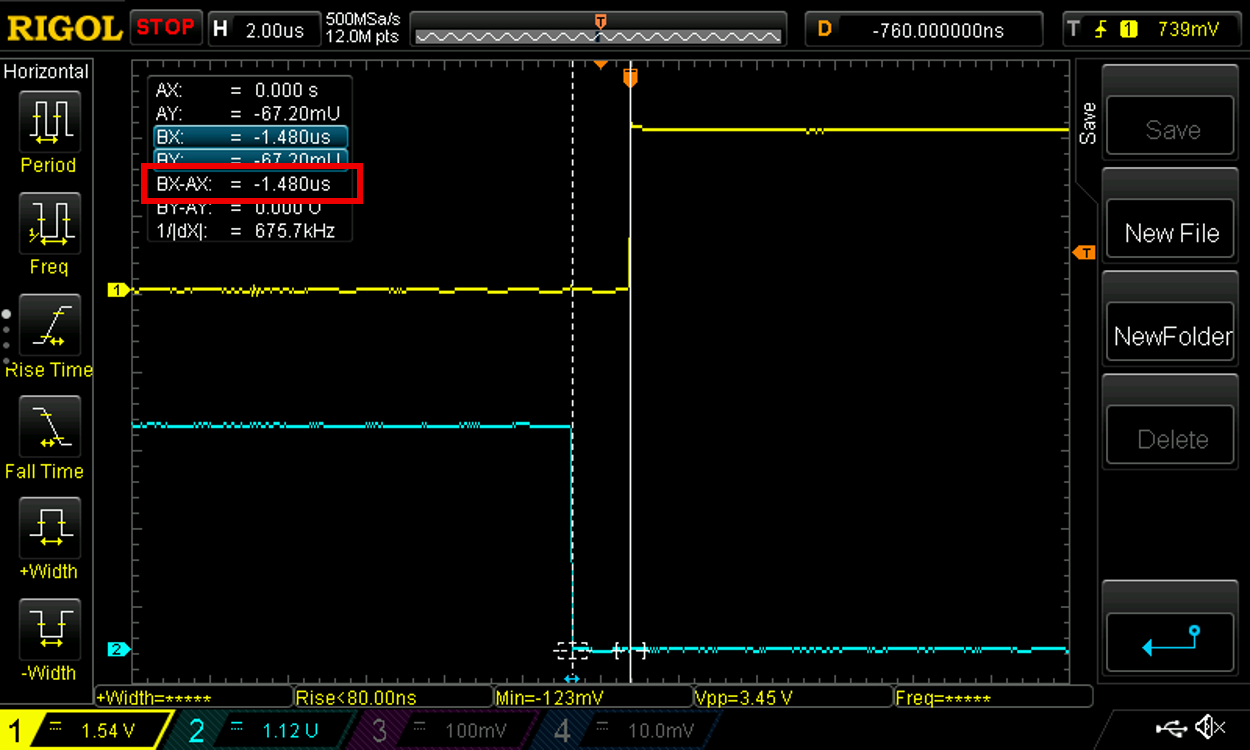
\includegraphics[width=\textwidth]{gambar/stm32_deadtime}
    \caption{Tepi transisi pertama ($\approx$1,48~$\mu$s)}
    \label{fig:dead-time-1}
  \end{subfigure}\hfill
  \begin{subfigure}{0.49\textwidth}
    \centering
    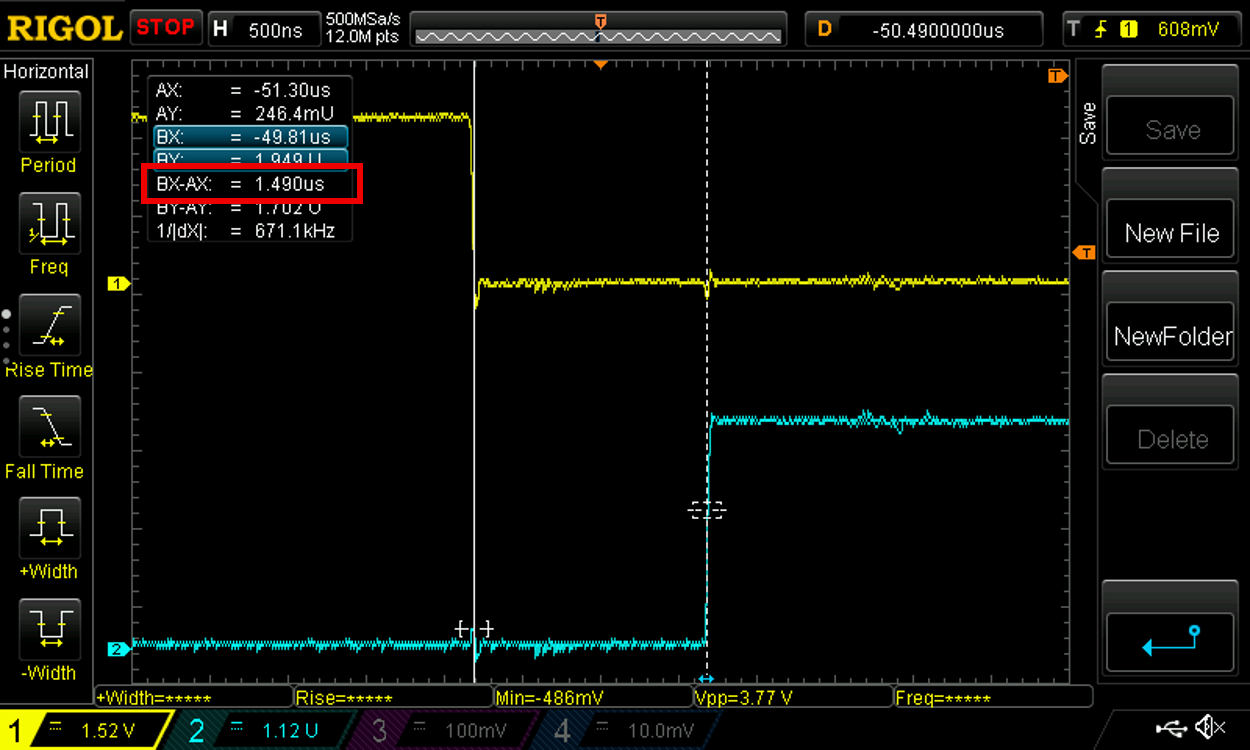
\includegraphics[width=\textwidth]{gambar/stm32_deadtime_2}
    \caption{Tepi transisi kedua ($\approx$1,49~$\mu$s)}
    \label{fig:dead-time-2}
  \end{subfigure}
  \caption{Pengukuran \emph{dead time} sinyal PWM komplementer STM32}
  \label{fig:dead-time}
\end{figure}

\begin{table}[H]
\centering
\caption{Pengujian sinyal PWM dan sinyal komplementer}
\label{tab:pwm-komplementer}
  \begin{tabularx}{\linewidth}{|c|>{\centering\arraybackslash\hsize=0.7\hsize}X|>{\raggedright\arraybackslash\hsize=1.5\hsize}X|>{\centering\arraybackslash\hsize=0.8\hsize}X|}
\hline
\textbf{No.} &
\textbf{Pin} &
\textbf{Kondisi Sinyal} &
\textbf{\emph{Dead Time}} \\
\hline
1 & PA8 & PWM utama & 1,48~$\mu$s \\
\hline
2 & PA7 & PWM komplementer (berlawanan fasa) & 1,49~$\mu$s \\
\hline
\end{tabularx}
\end{table}


\begin{figure}[H]
  \centering
  \begin{subfigure}{0.49\textwidth}
    \centering
    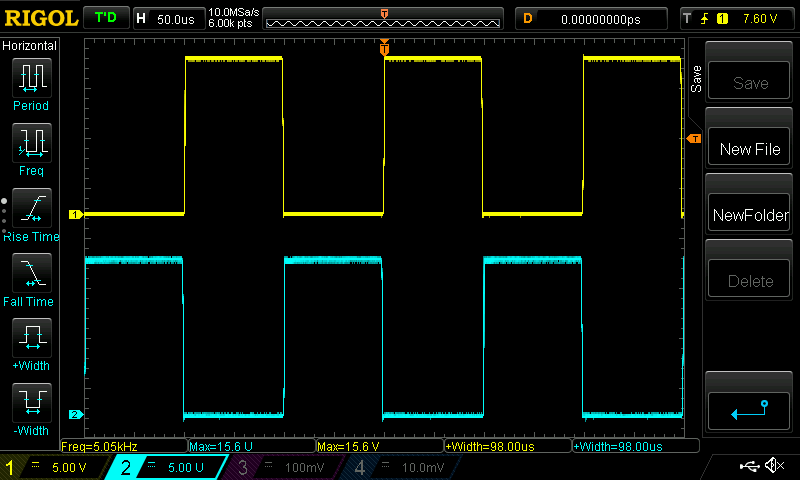
\includegraphics[width=\textwidth]{gambar/pwm_driver_dc50}
    \caption{\emph{Duty cycle} 50\%}
    \label{fig:pwm-driver-dc50}
  \end{subfigure}\hfill
  \begin{subfigure}{0.49\textwidth}
    \centering
    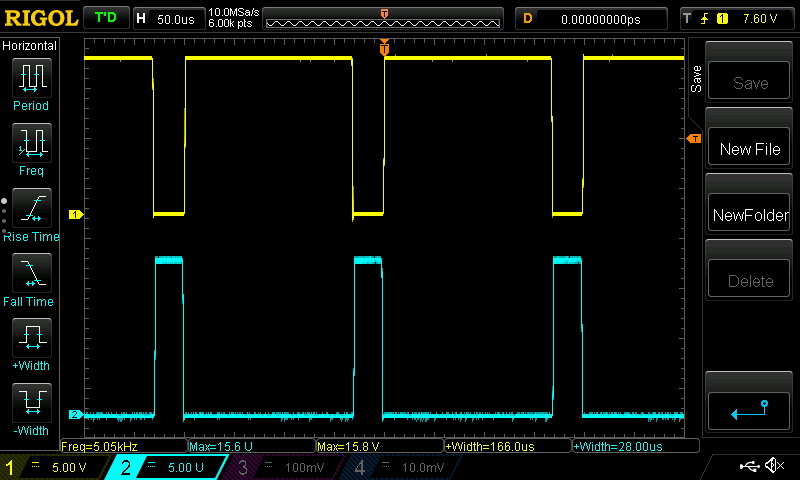
\includegraphics[width=\textwidth]{gambar/pwm_driver_dc85}
    \caption{\emph{Duty cycle} 85\%}
    \label{fig:pwm-driver-dc85}
  \end{subfigure}
  \caption{Keluaran \emph{gate driver} HCPL-3120 (sepasang sinyal komplementer
  dengan amplitudo gerbang $\approx$15,6~V)}
  \label{fig:pwm-driver}
\end{figure}

\begin{figure}[H]
  \centering
  \begin{subfigure}{0.49\textwidth}
    \centering
    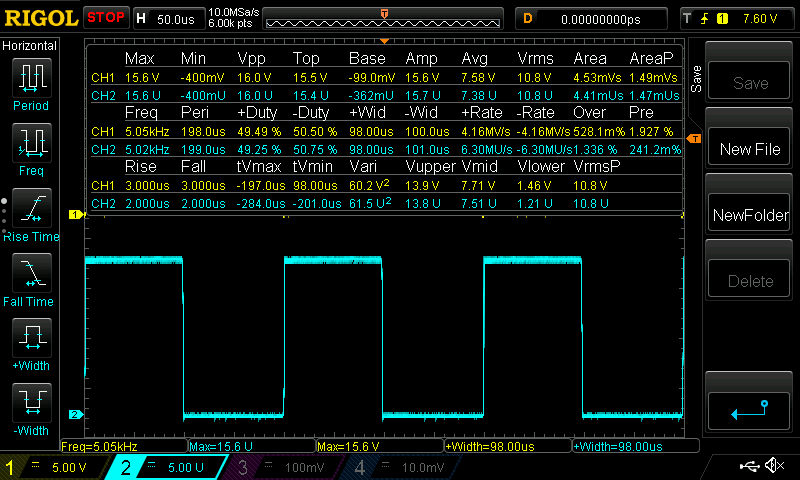
\includegraphics[width=\textwidth]{gambar/pwm_driver_dc50_measure}
    \caption{\emph{Duty cycle} 50\%}
    \label{fig:pwm-driver-dc50-m}
  \end{subfigure}\hfill
  \begin{subfigure}{0.49\textwidth}
    \centering
    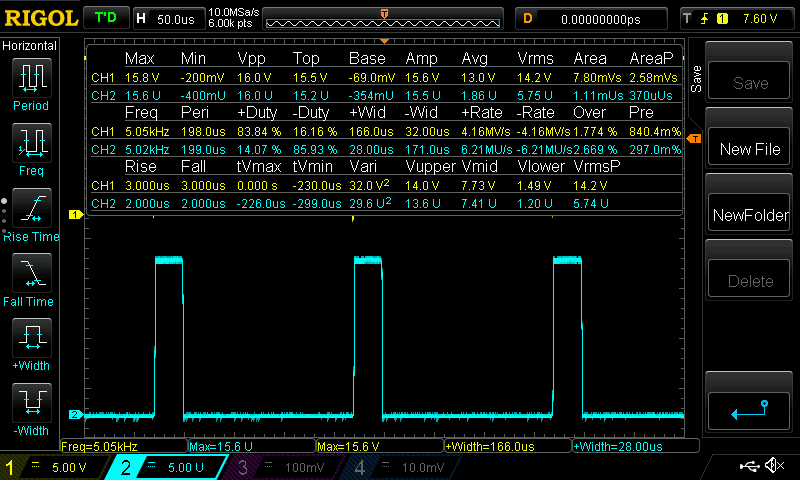
\includegraphics[width=\textwidth]{gambar/pwm_driver_dc85_measure}
    \caption{\emph{Duty cycle} 85\%}
    \label{fig:pwm-driver-dc85-m}
  \end{subfigure}
  \caption{Pengukuran rinci keluaran \emph{gate driver} HCPL-3120}
  \label{fig:pwm-driver-measure}
\end{figure}

\begin{figure}[H]
  \centering
  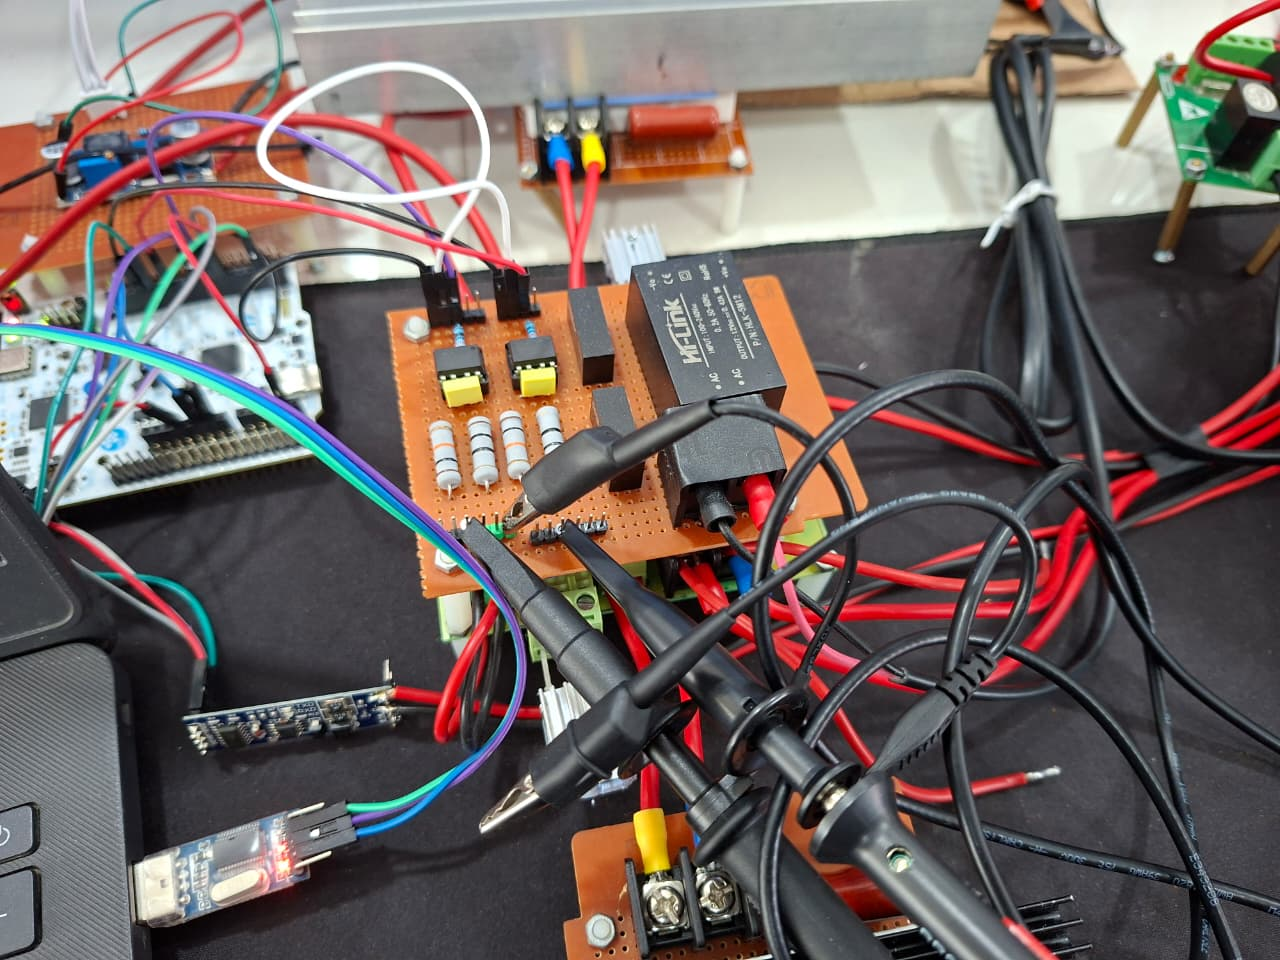
\includegraphics[width=0.50\textwidth]{gambar/uji_pwm_driver}
  \caption{Dokumentasi pengujian keluaran \emph{gate driver} HCPL-3120}
  \label{fig:uji-pwm-driver}
\end{figure}


Selanjutnya, keluaran \emph{gate driver} optocoupler HCPL-3120 diamati untuk
memastikan sinyal PWM dari STM32 (level logika 3,3~V) dikuatkan menjadi level
tegangan gerbang yang sesuai untuk memicu IGBT, dengan bentuk dan \emph{duty
cycle} yang tetap terjaga. Hasil pengamatan pada \emph{duty cycle} 50\% dan
85\% ditunjukkan pada Gambar~\ref{fig:pwm-driver}, sedangkan pengukuran
rincinya pada Gambar~\ref{fig:pwm-driver-measure}.

Berdasarkan Tabel~\ref{tab:hasil-pwm-stm32}, \emph{duty cycle} sinyal aktif
(PA8) terukur sangat dekat dengan nilai yang diatur pada seluruh rentang
10--95\% (selisih $\leq$1\%), sedangkan sinyal \emph{freewheeling} (PA7)
bersifat komplementer terhadapnya. Jumlah \emph{duty cycle} PA8 dan PA7
mendekati 99\% (bukan tepat 100\%) karena adanya \emph{dead time} di kedua tepi
transisi, yang konsisten dengan hasil pengukuran \emph{dead time} 1,48--1,49~$\mu$s.
Frekuensi PWM terukur 5,05~kHz (target 5~kHz, selisih $\approx$1\%). Pada sisi
keluaran, \emph{gate driver} HCPL-3120 mempertahankan bentuk dan \emph{duty
cycle} sinyal (mis. 49,5\% dan 83,8\%) serta menaikkan amplitudo menjadi
$\approx$15,6~V yang memadai untuk memicu IGBT. Dengan demikian, rantai
pembangkitan sinyal kendali dari STM32 hingga \emph{gate driver} telah bekerja
sesuai rancangan.

\section{Pengujian Sensor Tekanan Air}
\label{sec:pengujian-sensor-tekanan}

Pengujian sensor tekanan air dilakukan untuk memastikan pembacaan ADC pada
STM32 dapat dikonversi menjadi nilai tekanan yang sesuai. Sensor yang digunakan
memiliki rentang tegangan keluaran 0,5 V sampai 4,5 V untuk rentang tekanan
0 bar sampai 12 bar. Karena tegangan maksimum sensor lebih besar dari tegangan
masukan ADC STM32, digunakan rangkaian pembagi tegangan sebelum sinyal masuk
ke pin ADC. Rangkaian pembagi tegangan ini menurunkan tegangan sensor sehingga 
berada dalam rentang 0--3,3 V yang aman untuk ADC.
Nilai resistor yang digunakan pada pembagi tegangan adalah R1 = 10 k$\Omega$ dan R2 = 20 k$\Omega$.

Grafik karakteristik sensor tekanan air ditunjukkan pada Gambar~\ref{fig:grafik-sensor-adc}.
Hasil pembacaan sensor tekanan air ditunjukkan pada Tabel~\ref{tab:hasil-sensor-tekanan}.

\begin{table}[H]
\centering
\caption{Hasil pembacaan sensor tekanan air}
\label{tab:hasil-sensor-tekanan}
\small
\renewcommand{\arraystretch}{1.1}
\begin{tabularx}{\linewidth}{|c|>{\centering\arraybackslash}X|>{\centering\arraybackslash}X|>{\centering\arraybackslash}X|>{\centering\arraybackslash}X|}
\hline
\textbf{No.} &
\textbf{Nilai Bit ADC} &
\textbf{$V_{\text{ADC}}$ (V)} &
\textbf{$V_{\text{Sensor}}$ (V)} &
\textbf{Tekanan (bar)} \\
\hline
1  & 429 & 0,3348 & 0,4933 & 0,009 \\ \hline
2  & 421 & 0,3333 & 0,4937 & 0,012 \\ \hline
3  & 442 & 0,3472 & 0,5080 & 0,035 \\ \hline
4  & 433 & 0,3512 & 0,5149 & 0,052 \\ \hline
5  & 446 & 0,3600 & 0,5247 & 0,081 \\ \hline
6  & 488 & 0,3757 & 0,5491 & 0,149 \\ \hline
7  & 487 & 0,3840 & 0,5593 & 0,180 \\ \hline
8  & 490 & 0,3872 & 0,5681 & 0,205 \\ \hline
9  & 539 & 0,3981 & 0,5815 & 0,244 \\ \hline
10 & 489 & 0,3990 & 0,5843 & 0,254 \\ \hline
11 & 524 & 0,4097 & 0,6011 & 0,303 \\ \hline
12 & 538 & 0,4203 & 0,6137 & 0,341 \\ \hline
13 & 540 & 0,4229 & 0,6171 & 0,352 \\ \hline
14 & 522 & 0,4301 & 0,6361 & 0,409 \\ \hline
15 & 582 & 0,4459 & 0,6473 & 0,442 \\ \hline
16 & 552 & 0,4439 & 0,6506 & 0,452 \\ \hline
17 & 572 & 0,4573 & 0,6709 & 0,513 \\ \hline
18 & 584 & 0,4631 & 0,6807 & 0,543 \\ \hline
19 & 587 & 0,4673 & 0,6851 & 0,556 \\ \hline
20 & 583 & 0,4715 & 0,6923 & 0,577 \\ \hline
21 & 699 & 0,4875 & 0,7145 & 0,643 \\ \hline
22 & 691 & 0,5113 & 0,7515 & 0,754 \\ \hline
23 & 602 & 0,5267 & 0,7814 & 0,844 \\ \hline
24 & 719 & 0,5444 & 0,7969 & 0,890 \\ \hline
25 & 690 & 0,5496 & 0,8095 & 0,929 \\ \hline
26 & 697 & 0,5544 & 0,8150 & 0,945 \\ \hline
\end{tabularx}
\end{table}
\renewcommand{\arraystretch}{1.4}

\begin{figure}[H]
\centering
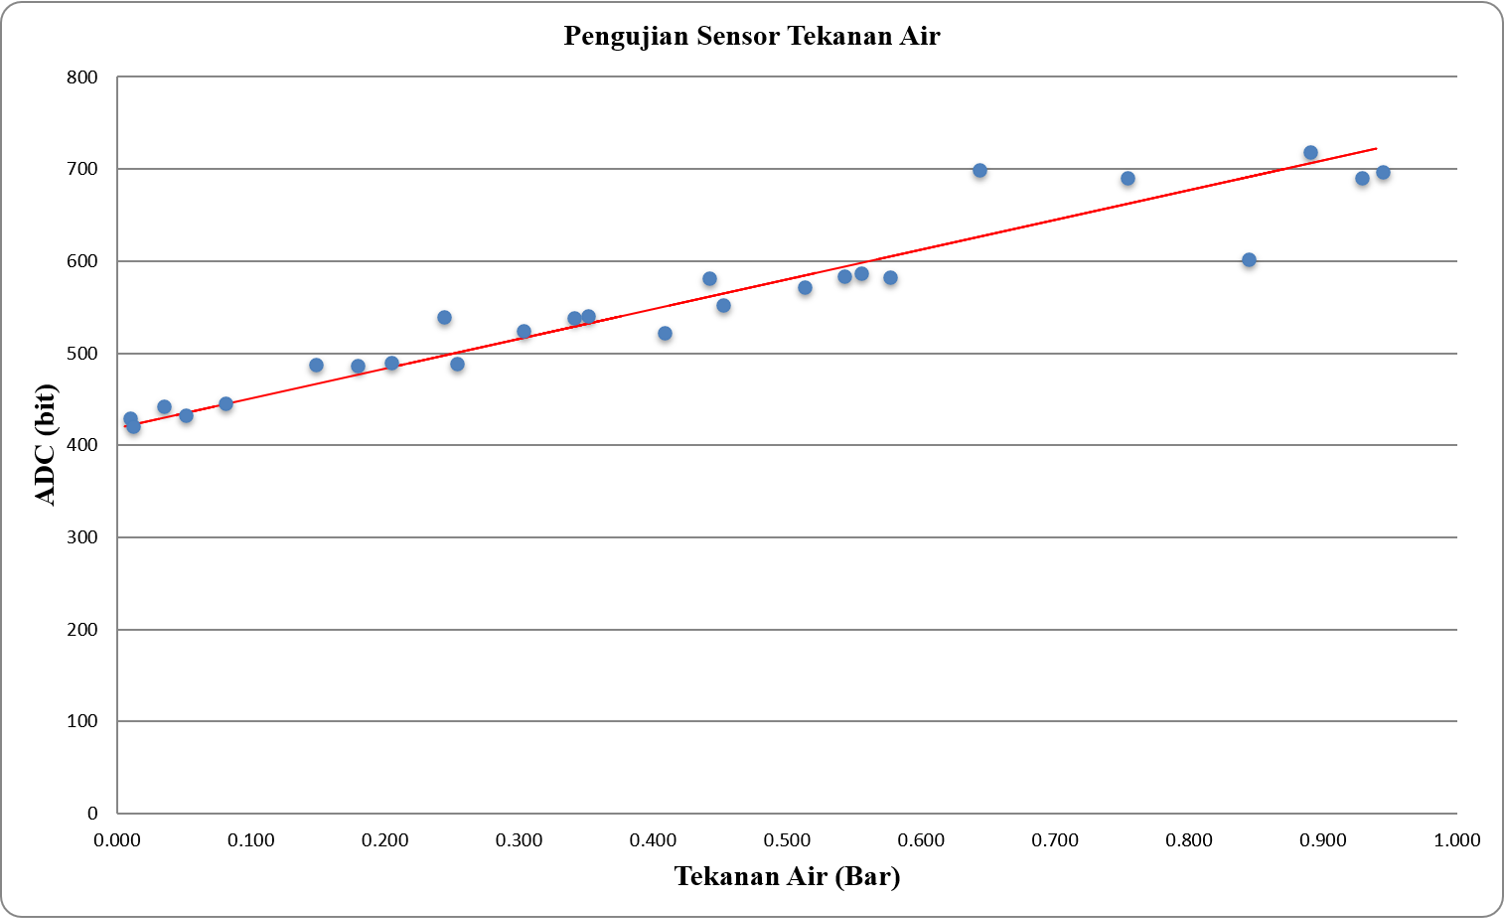
\includegraphics[width=0.55\textwidth]{gambar/pengujian_sensor_tekanan.png}
\caption{Grafik karakteristik sensor tekanan air: tekanan (bar) vs nilai bit ADC}
\label{fig:grafik-sensor-adc}
\end{figure}

\section{Pengujian Sistem PWM AC \emph{Chopper} dengan Beban Lampu}
\label{sec:pengujian-beban-lampu}

Pengujian dengan beban lampu dilakukan untuk memvalidasi kemampuan
rangkaian PWM AC \emph{chopper} dalam mengatur tegangan keluaran sebelum
diuji dengan beban pompa air. Dokumentasi pengujian dan hasil pengukuran
tegangan ditunjukkan pada Gambar~\ref{fig:uji-lampu-1} dan
Gambar~\ref{fig:uji-lampu-2}. Gambar utama pengujian lampu ditunjukkan pada Gambar~\ref{fig:uji-lampu}.

\begin{figure}[H]
  \centering
  \begin{subfigure}{0.58\textwidth}
    \centering
    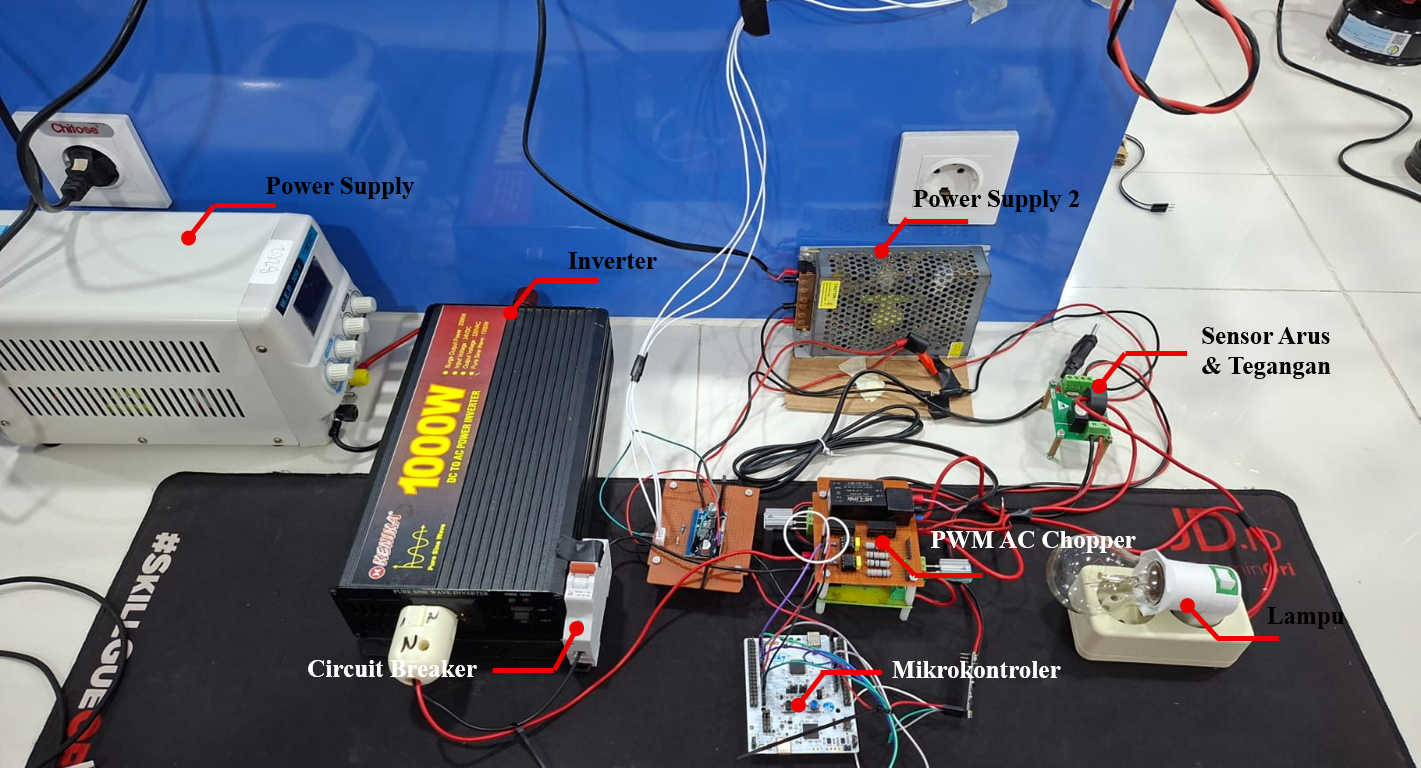
\includegraphics[width=\textwidth]{gambar/uji_lampu.png}
    \caption{}
    \label{fig:uji-lampu-1}
  \end{subfigure}

  \vspace{0.5em}

  \begin{subfigure}{0.58\textwidth}
    \centering
    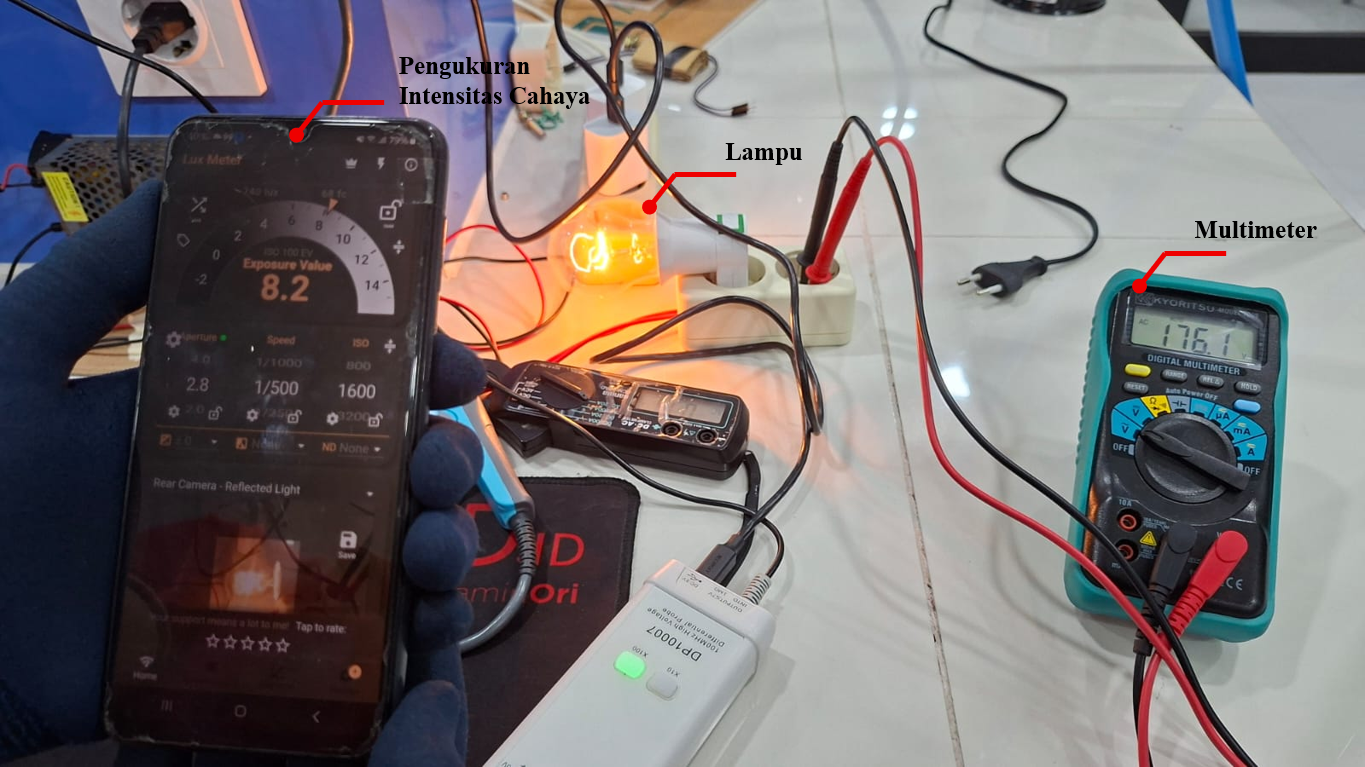
\includegraphics[width=\textwidth]{gambar/uji_lampu2.png}
    \caption{}
    \label{fig:uji-lampu-2}
  \end{subfigure}
  \caption{Pengujian PWM AC \emph{chopper}: (a) dengan beban lampu dan (b) pengukuran intensitas cahaya dan tegangan RMS keluaran.}
  \label{fig:uji-lampu}
\end{figure}

Pengujian dengan beban lampu pijar 10~W dilakukan untuk memverifikasi kemampuan
rangkaian PWM AC \emph{chopper} dalam mengatur tegangan keluaran sebelum
dihubungkan ke beban pompa air. Beban lampu dipilih karena bersifat resistif
murni sehingga hubungan antara \emph{duty cycle} dan tegangan RMS keluaran
dapat diamati secara langsung tanpa pengaruh komponen reaktif. Pada setiap
titik \emph{duty cycle}, tegangan RMS keluaran diukur menggunakan voltmeter
dan intensitas cahaya lampu dicatat melalui nilai \emph{exposure value} (EV)
sebagai indikator kualitatif perubahan daya. Hasil pengukuran ditunjukkan pada
Tabel~\ref{tab:duty-lampu}, sedangkan grafik hubungan \emph{duty cycle}
terhadap tegangan RMS keluaran ditunjukkan pada
Gambar~\ref{fig:grafik-lampu-duty}.

\begin{table}[H]
\centering
\caption{Hasil pengujian PWM AC \emph{chopper} dengan beban lampu pijar 10~W}
\label{tab:duty-lampu}
\small
\renewcommand{\arraystretch}{1.15}
\begin{tabularx}{\linewidth}{|c|>{\centering\arraybackslash}X|>{\centering\arraybackslash}X|>{\centering\arraybackslash}X|>{\centering\arraybackslash}X|>{\centering\arraybackslash}X|>{\centering\arraybackslash}X|}
\hline
\textbf{No.} &
\textbf{$V_{\text{input}}$ (V)} &
\textbf{\emph{Duty Cycle} (\%)} &
\textbf{$V_{\text{teoritis}}$ (V)} &
\textbf{$V_{\text{terukur}}$ (V)} &
\textbf{Error (\%)} &
\textbf{EV} \\
\hline
1  & 220 & 25 & 55,00  & 38,48  & 30,04 & 6,9 \\ \hline
2  & 220 & 30 & 66,00  & 65,10  & 1,36  & 7,3 \\ \hline
3  & 220 & 35 & 77,00  & 75,90  & 1,43  & 7,3 \\ \hline
4  & 220 & 40 & 88,00  & 87,00  & 1,14  & 7,5 \\ \hline
5  & 220 & 45 & 99,00  & 98,40  & 0,61  & 7,3 \\ \hline
6  & 220 & 50 & 110,00 & 109,50 & 0,45  & 7,6 \\ \hline
7  & 220 & 55 & 121,00 & 120,50 & 0,41  & 7,8 \\ \hline
8  & 220 & 60 & 132,00 & 131,60 & 0,30  & 7,9 \\ \hline
9  & 220 & 65 & 143,00 & 142,60 & 0,28  & 8,0 \\ \hline
10 & 220 & 70 & 154,00 & 153,70 & 0,19  & 8,0 \\ \hline
11 & 220 & 75 & 165,00 & 164,90 & 0,06  & 8,2 \\ \hline
12 & 220 & 80 & 176,00 & 176,10 & 0,06  & 8,2 \\ \hline
13 & 220 & 85 & 187,00 & 187,20 & 0,11  & 8,3 \\ \hline
14 & 220 & 90 & 198,00 & 198,30 & 0,15  & 8,4 \\ \hline
15 & 220 & 95 & 209,00 & 209,50 & 0,24  & 8,5 \\ \hline
\end{tabularx}
\end{table}
\renewcommand{\arraystretch}{1.4}

\begin{figure}[H]
\centering
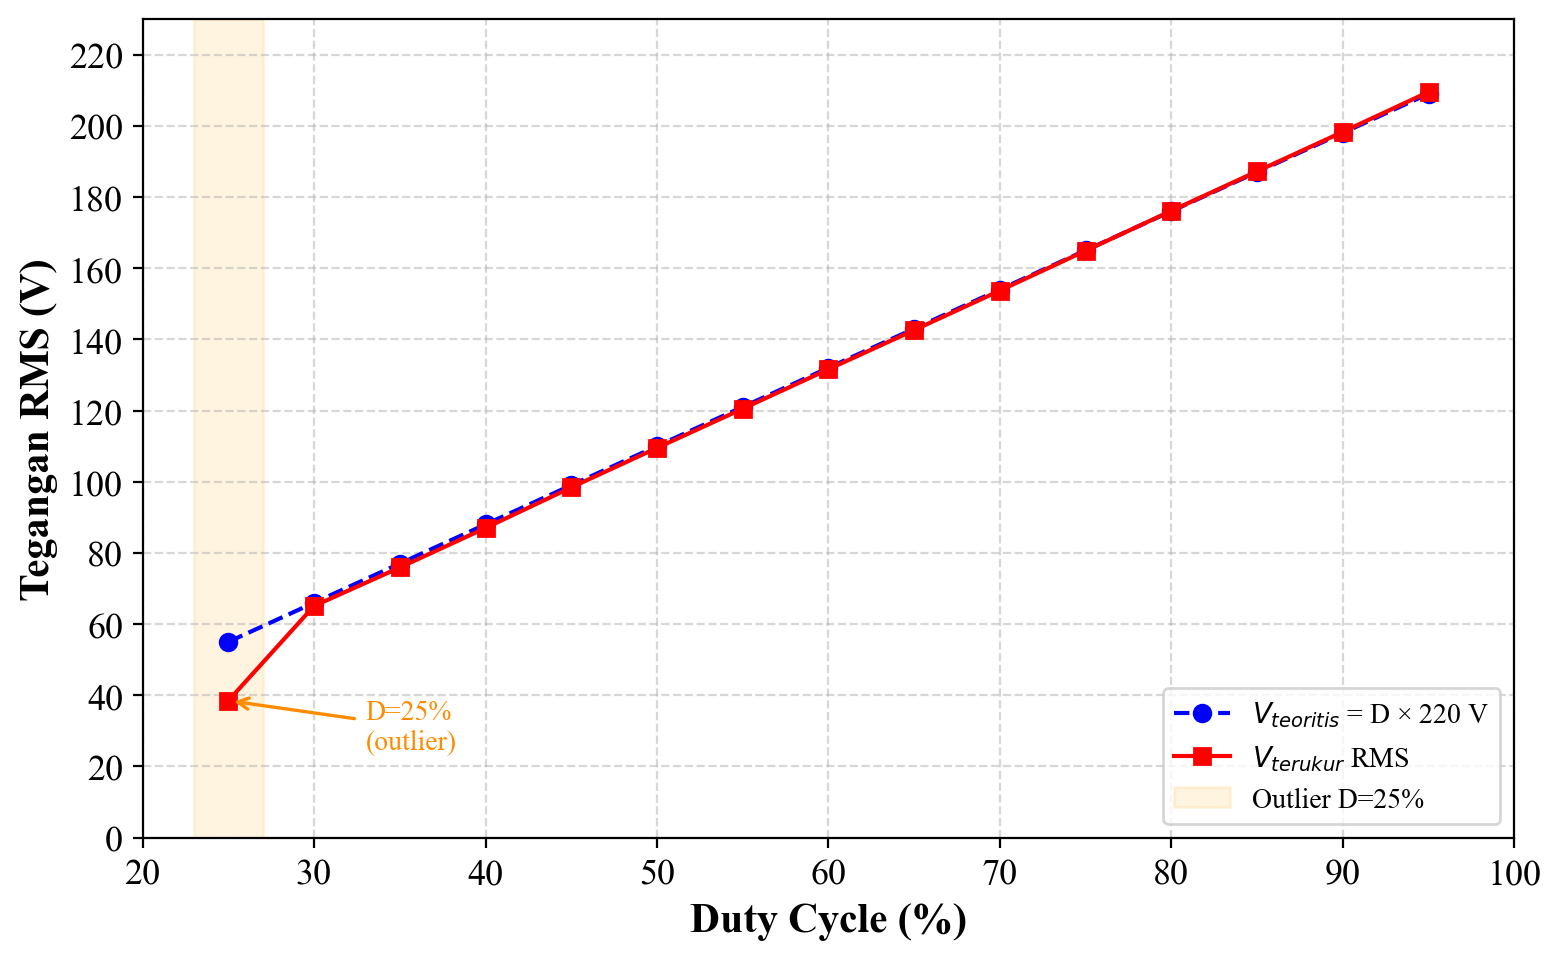
\includegraphics[width=0.65\textwidth]{gambar/grafik_lampu_duty_tegangan}
\caption{Grafik hubungan \emph{duty cycle} dan tegangan keluaran RMS pada beban lampu pijar 10~W}
\label{fig:grafik-lampu-duty}
\end{figure}

Data di atas menunjukkan perbandingan antara tegangan teoritis
($V_{\text{teoritis}} = D \times V_{\text{in}}$, dengan $V_{\text{in}} = 220$~V)
dan tegangan RMS terukur pada setiap titik \emph{duty cycle}.
Pada rentang \emph{duty} 30--95\%, \emph{error} berkisar antara 0,06\% hingga
1,43\%, yang menunjukkan linearitas keluaran yang sangat baik dan memvalidasi
bahwa rangkaian PWM AC \emph{chopper} bekerja sesuai model teoritis.
Pada \emph{duty} 25\%, \emph{error} mencapai 30,04\% karena tegangan terukur
hanya 38,48~V, jauh di bawah nilai teoritis 55,00~V. Hal ini disebabkan oleh
efek \emph{dead time} (1,5~$\mu$s) dan ambang konduksi IGBT yang menjadi
signifikan pada \emph{duty cycle} sangat rendah, sehingga titik kerja minimum
sistem secara efektif dimulai dari \emph{duty} 30\%.
Nilai \emph{exposure value} juga meningkat seiring naiknya \emph{duty cycle},
dari EV 6,9 pada \emph{duty} 25\% menjadi EV 8,5 pada \emph{duty} 95\%,
mengonfirmasi bahwa daya yang diserap lampu bertambah secara konsisten.
Secara keseluruhan, hasil pengujian ini memvalidasi bahwa rangkaian PWM AC
\emph{chopper} mampu mengatur tegangan keluaran secara akurat pada rentang
operasi efektif 30--95\% sebelum diterapkan pada beban pompa air.

\section{Pengujian Sistem PWM AC \emph{Chopper} dengan Beban Pompa Air}
\label{sec:pengujian-beban-pompa}

Pengujian dengan beban pompa air dilakukan untuk mengetahui karakteristik
kelistrikan beban pompa ketika \emph{duty cycle} PWM divariasikan. Pada setiap
titik \emph{duty cycle}, tegangan RMS keluaran dan arus beban diukur
menggunakan \emph{power meter} JSY. Dokumentasi pengujian ditunjukkan pada
Gambar~\ref{fig:uji-pompa-1}.

\begin{figure}[H]
  \centering
  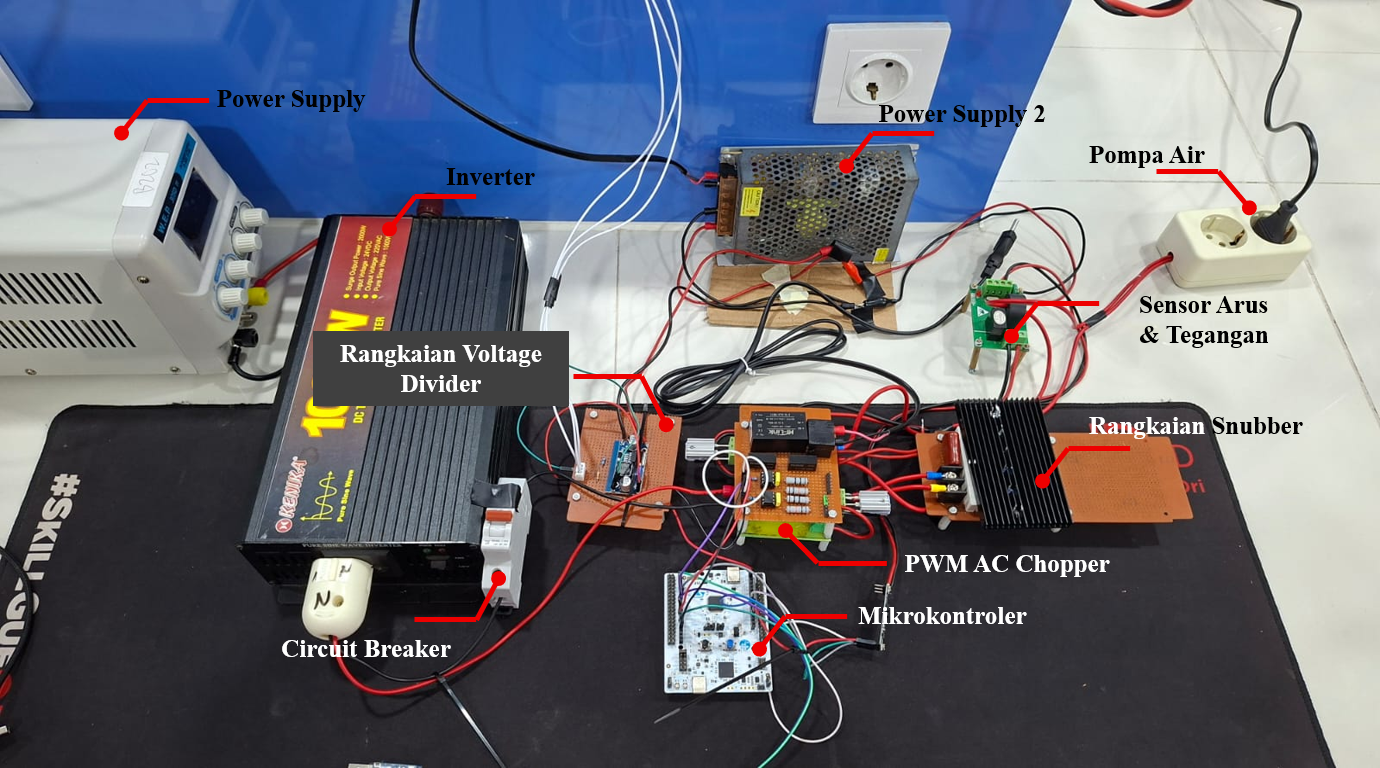
\includegraphics[width=0.65\textwidth]{gambar/uji_pompa.png}
  \caption{Pengujian PWM AC \emph{chopper} dengan beban pompa air.}
  \label{fig:uji-pompa-1}
\end{figure}

Sistem pipa dan keran yang digunakan
ditunjukkan pada Gambar~\ref{fig:uji-pompa-2}, hasil pengukuran
ditunjukkan pada Tabel~\ref{tab:duty-tekanan-pompa}, dan grafik hubungannya
pada Gambar~\ref{fig:grafik-pompa-duty}. Tekanan air tidak
ditampilkan sebagai fungsi tunggal \emph{duty cycle} karena tekanan juga
bergantung pada jumlah keran terbuka (beban hidraulik); hubungan tekanan
terhadap kendali dibahas pada Subbab~\ref{sec:pengujian-sistem-kendali}.

\begin{figure}[H]
  \centering
  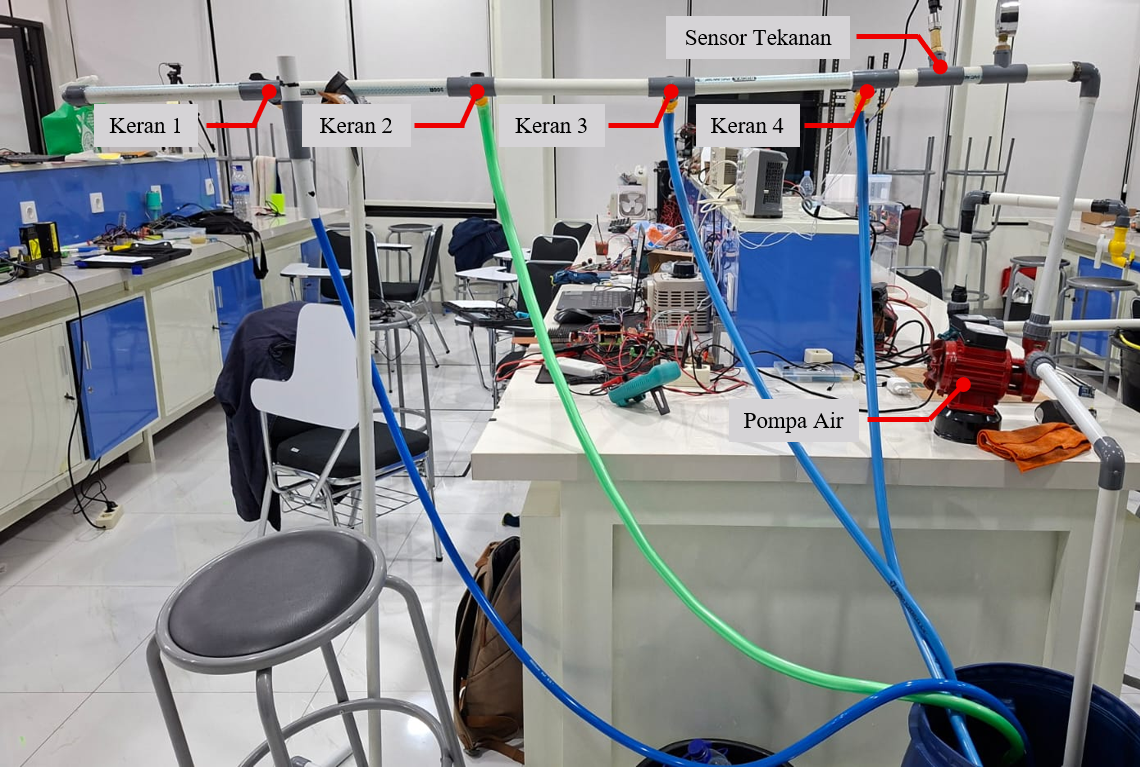
\includegraphics[width=0.65\textwidth]{gambar/uji_pompa2.png}
  \caption{Sistem pipa dan keran pada pengujian beban pompa air.}
  \label{fig:uji-pompa-2}
\end{figure}

\begin{table}[H]
\centering
\caption{Karakteristik elektrik beban pompa terhadap \emph{duty cycle}}
\label{tab:duty-tekanan-pompa}
  \begin{tabularx}{\linewidth}{|c|>{\centering\arraybackslash}X|>{\centering\arraybackslash}X|>{\centering\arraybackslash}X|>{\centering\arraybackslash}X|>{\centering\arraybackslash}X|}
\hline
\textbf{No.} &
\textbf{$V_{\text{input}}$ (V)} &
\textbf{\emph{Duty} (\%)} &
\textbf{$V_{\text{teoritis}}$ (V)} &
\textbf{$V_{\text{out}}$ RMS (V)} &
\textbf{Error (\%)} \\
\hline
1 & 220 & 70 & 154,00 & 155,5 & 0,97 \\ \hline
2 & 220 & 75 & 165,00 & 164,5 & 0,30 \\ \hline
3 & 220 & 80 & 176,00 & 174,9 & 0,62 \\ \hline
4 & 220 & 85 & 187,00 & 185,7 & 0,70 \\ \hline
5 & 220 & 90 & 198,00 & 196,6 & 0,71 \\ \hline
6 & 220 & 95 & 209,00 & 207,3 & 0,81 \\ \hline
\end{tabularx}
\end{table}

\begin{figure}[H]
\centering
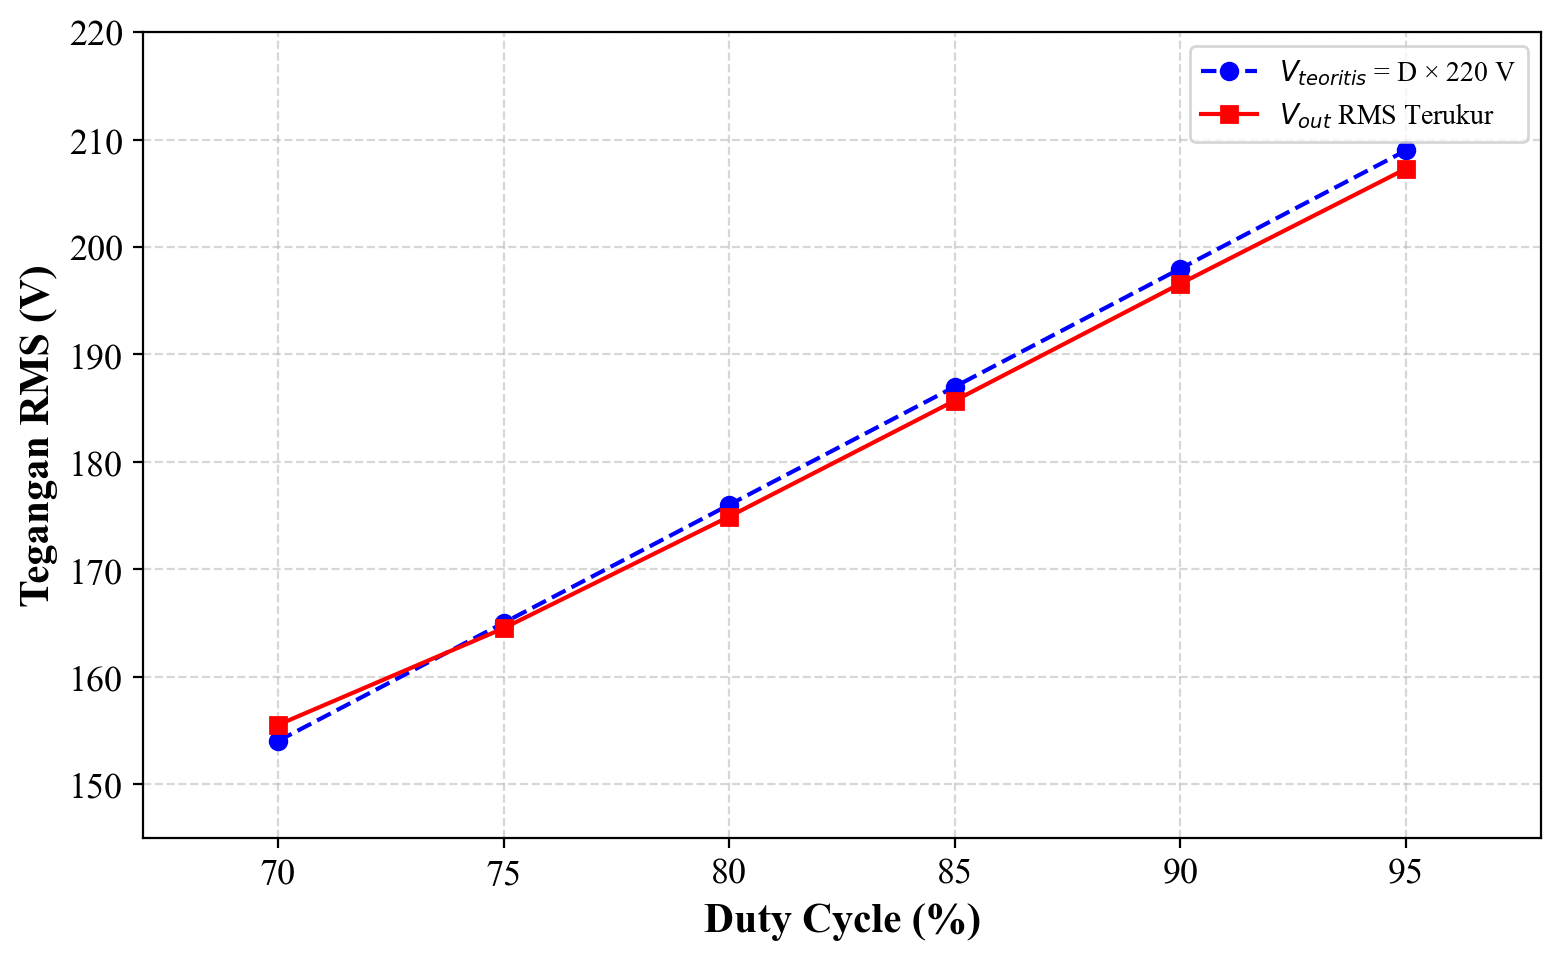
\includegraphics[width=0.65\textwidth]{gambar/grafik_pompa_duty_tegangan}
\caption{Grafik hubungan \emph{duty cycle} dan tegangan keluaran RMS pada beban pompa air}
\label{fig:grafik-pompa-duty}
\end{figure}

Data di atas menunjukkan bahwa kenaikan \emph{duty cycle}
meningkatkan tegangan RMS keluaran secara hampir linear, dari 155,5~V pada
\emph{duty} 70\% menjadi 207,3~V pada \emph{duty} 95\%.
\emph{Error} terhadap nilai teoritis ($V_{\text{teoritis}} = D \times V_{\text{in}}$)
berada pada rentang 0,30\%--0,97\%, yang mengonfirmasi linearitas keluaran yang sangat
baik pada seluruh rentang kerja pompa (70--95\%). Arus beban berada pada
rentang 0,76--0,83~A, jauh di bawah kapasitas arus IGBT, sehingga rangkaian daya
mampu mengatur tegangan keluaran pompa secara aman pada seluruh rentang
\emph{duty cycle} kerja. Sehingga, pengujian ini memvalidasi bahwa sistem PWM AC \emph{chopper} dapat
mengatur tegangan keluaran pompa air pada rentang \emph{duty cycle} 70--95\% secara akurat.

\section{Perbandingan Hasil Simulasi dan Implementasi}
\label{sec:perbandingan-simulasi-implementasi}

Bagian ini membandingkan bentuk gelombang tegangan dan arus keluaran PWM AC
\emph{chopper} antara hasil simulasi PSIM (Subbab~\ref{sec:simulasi-psim}) dan
hasil pengukuran pada perangkat keras (osiloskop), pada rentang \emph{duty
cycle} kerja 70--95\%. Tujuannya adalah memvalidasi kesesuaian antara model
simulasi dan implementasi nyata.

% Helper subgambar perbandingan: tinggi seragam, rasio aspek terjaga
\newcommand{\cmpsub}[2]{%
  \begin{subfigure}{0.49\textwidth}\centering
    \includegraphics[width=\linewidth,height=3.6cm,keepaspectratio]{gambar/#1}
    \caption{#2}
  \end{subfigure}}

\subsection{Perbandingan Tegangan Keluaran PWM AC \emph{Chopper}}
\label{sec:banding-tegangan}

Pengukuran bentuk gelombang tegangan keluaran dilakukan menggunakan probe
\emph{isolated} (diferensial) untuk menghindari hubung singkat akibat tegangan
referensi rangkaian daya yang tidak berbasis ground yang sama. Dokumentasi
proses pengukuran ditunjukkan pada Gambar~\ref{fig:uji-voltage}. Selain itu,
Perbandingan bentuk gelombang tegangan keluaran ditunjukkan pada
Gambar~\ref{fig:banding-v-1}--\ref{fig:banding-v-3}.

\begin{figure}[H]
  \centering
  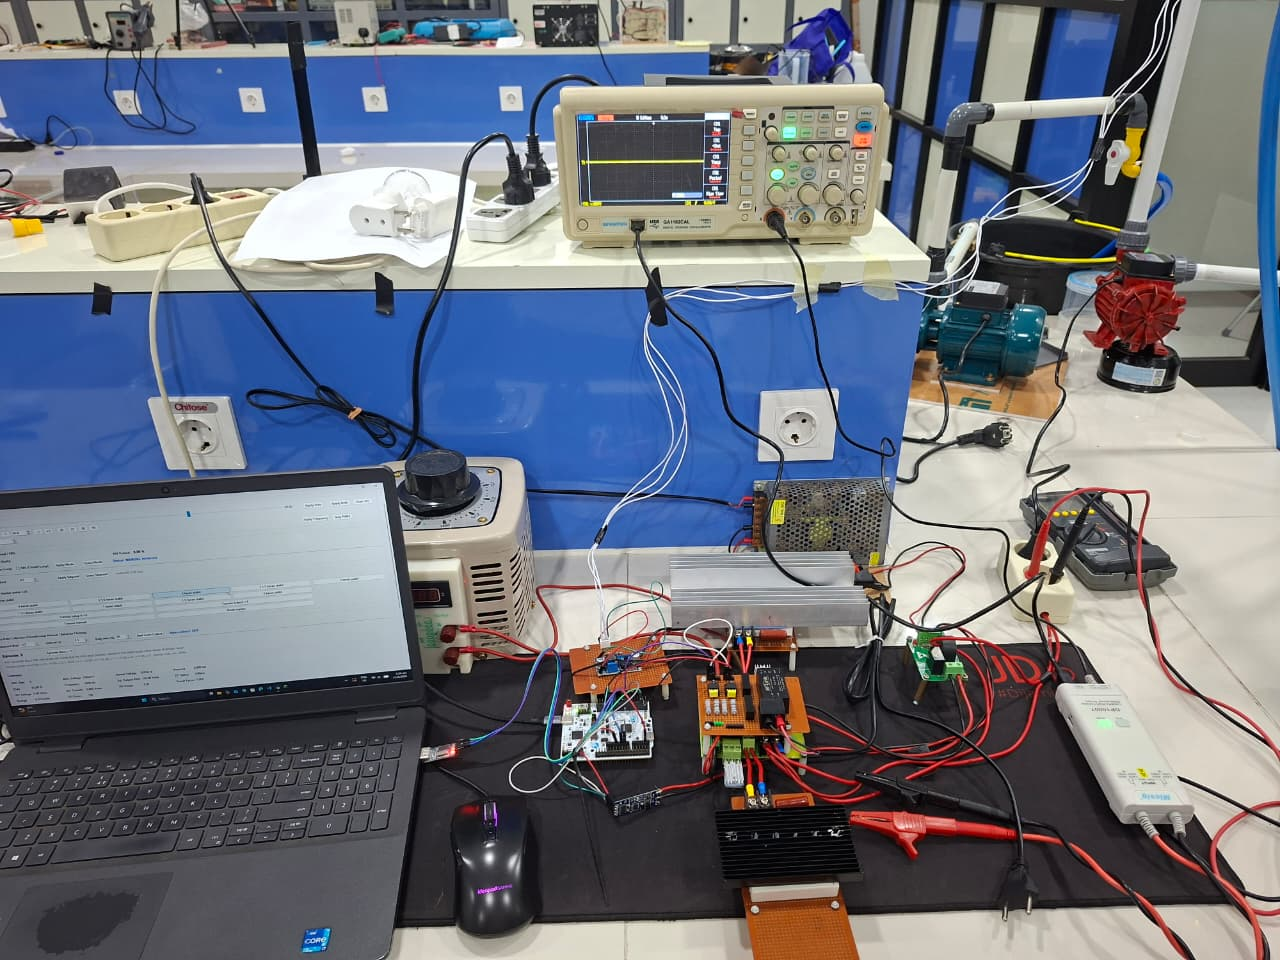
\includegraphics[width=0.58\textwidth]{gambar/uji_voltage}
  \caption{Pengukuran bentuk gelombang tegangan keluaran PWM AC \emph{chopper}
  menggunakan probe \emph{isolated}}
  \label{fig:uji-voltage}
\end{figure}

\begin{figure}[H]
  \centering
  \cmpsub{v_70}{70\% (terukur)}\hfill\cmpsub{v_70_s}{70\% (simulasi)}\par\medskip
  \cmpsub{v_75}{75\% (terukur)}\hfill\cmpsub{v_75_s}{75\% (simulasi)}
  \caption{Perbandingan tegangan keluaran terukur dan simulasi pada \emph{duty
  cycle} 70\% dan 75\%}
  \label{fig:banding-v-1}
\end{figure}

\begin{figure}[H]
  \centering
  \cmpsub{v_80}{80\% (terukur)}\hfill\cmpsub{v_80_s}{80\% (simulasi)}\par\medskip
  \cmpsub{v_85}{85\% (terukur)}\hfill\cmpsub{v_85_s}{85\% (simulasi)}
  \caption{Perbandingan tegangan keluaran terukur dan simulasi pada \emph{duty
  cycle} 80\% dan 85\%}
  \label{fig:banding-v-2}
\end{figure}


\begin{figure}[H]
  \centering
  \cmpsub{v_90}{90\% (terukur)}\hfill\cmpsub{v_90_s}{90\% (simulasi)}\par\medskip
  \cmpsub{v_95}{95\% (terukur)}\hfill\cmpsub{v_95_s}{95\% (simulasi)}
  \caption{Perbandingan tegangan keluaran terukur dan simulasi pada \emph{duty
  cycle} 90\% dan 95\%}
  \label{fig:banding-v-3}
\end{figure}

Bentuk gelombang tegangan keluaran hasil pengukuran sangat mirip dengan hasil
simulasi PSIM. Keduanya berupa gelombang sinus 50~Hz yang terpotong-potong
(\emph{chopped}) oleh PWM 5~kHz, dengan amplitudo selubung (\emph{envelope})
sinusoidal yang meningkat seiring kenaikan \emph{duty cycle} dan mencapai puncak
$\approx\pm220$~V pada \emph{duty} tinggi. Kesesuaian bentuk dan amplitudo ini
memperkuat validitas rancangan secara kuantitatif.

Dari hasil pengamatan bentuk gelombang, pada \emph{duty cycle} 70--85\%
teridentifikasi \emph{voltage spike} kecil pada tepi peralihan sinyal PWM.
\emph{Spike} ini merupakan akibat dari energi induktansi parasitik yang
terlepas saat IGBT memutus arus, namun amplitudonya masih berada di bawah
tegangan \emph{collector-emitter} maksimum ($V_{CE,max}$) IGBT FGH40N120AN
sehingga tidak membahayakan komponen. Rangkaian \emph{snubber} RC yang terpasang
berfungsi meredam lonjakan tersebut. Pada \emph{duty cycle} 90\% ke atas,
\emph{spike} tegangan tidak lagi teramati secara signifikan pada gelombang
keluaran yang masuk ke beban pompa, sehingga bentuk gelombang dapat dikatakan
bersih dan aman untuk operasi pompa.

\subsection{Perbandingan Arus Beban}
\label{sec:banding-arus}

Perbandingan bentuk gelombang arus beban ditunjukkan pada
Gambar~\ref{fig:banding-i-1}--\ref{fig:banding-i-3}. Perbandingan arus pada
\emph{duty cycle} 70\% dan 75\% ditunjukkan pada Gambar~\ref{fig:banding-i-1},
perbandingan arus pada \emph{duty cycle} 80\% dan 85\% ditunjukkan pada
Gambar~\ref{fig:banding-i-2}, sedangkan perbandingan arus pada \emph{duty
cycle} 90\% dan 95\% ditunjukkan pada Gambar~\ref{fig:banding-i-3}. Pola
kenaikan amplitudo arus terhadap \emph{duty cycle} pada ketiga pasang gambar
tersebut konsisten dengan kenaikan tegangan keluaran yang telah dibahas
sebelumnya.

\begin{figure}[H]
  \centering
  \cmpsub{i_70}{70\% (terukur)}\hfill\cmpsub{i2_70}{70\% (simulasi)}\par\medskip
  \cmpsub{i_75}{75\% (terukur)}\hfill\cmpsub{i2_75}{75\% (simulasi)}
  \caption{Perbandingan arus beban terukur dan simulasi pada \emph{duty cycle}
  70\% dan 75\%}
  \label{fig:banding-i-1}
\end{figure}

\begin{figure}[H]
  \centering
  \cmpsub{i_80}{80\% (terukur)}\hfill\cmpsub{i2_80}{80\% (simulasi)}\par\medskip
  \cmpsub{i_85}{85\% (terukur)}\hfill\cmpsub{i2_85}{85\% (simulasi)}
  \caption{Perbandingan arus beban terukur dan simulasi pada \emph{duty cycle}
  80\% dan 85\%}
  \label{fig:banding-i-2}
\end{figure}

\begin{figure}[H]
  \centering
  \cmpsub{i_90}{90\% (terukur)}\hfill\cmpsub{i2_90}{90\% (simulasi)}\par\medskip
  \cmpsub{i_95}{95\% (terukur)}\hfill\cmpsub{i2_95}{95\% (simulasi)}
  \caption{Perbandingan arus beban terukur dan simulasi pada \emph{duty cycle}
  90\% dan 95\%}
  \label{fig:banding-i-3}
\end{figure}

Bentuk gelombang arus beban hasil pengukuran maupun simulasi sama-sama mendekati
sinusoidal akibat sifat induktif motor pompa, dengan riak (\emph{ripple})
\emph{switching} pada frekuensi PWM yang tampak pada kedua hasil. Amplitudo arus
puncak berada pada kisaran $\approx\pm1,2$~A. Nilai arus RMS terukur
(0,76--0,83~A, Tabel~\ref{tab:duty-tekanan-pompa}) konsisten dengan amplitudo
hasil simulasi tersebut. 

\section{Pengambilan Dataset untuk \emph{Neural Network}}
\label{sec:dataset-neural-network}

Dataset \emph{neural network} diperoleh dari hasil pembacaan sistem saat pompa
diberi variasi \emph{duty cycle} dan variasi kondisi beban. Data yang direkam
meliputi waktu pengambilan data, nilai ADC, tekanan air, tegangan RMS keluaran,
\emph{duty cycle}, frekuensi PWM, dan kondisi beban. Dataset ini digunakan
sebagai dasar pelatihan dan pengujian model.

Pengambilan data dilakukan secara \emph{closed-loop} manual, yaitu operator
bertindak sebagai pengendali yang mengejar tekanan target 0,30~bar menggunakan
kebijakan proporsional sederhana, sementara sistem mencatat setiap keputusan
koreksi yang diambil. Pendekatan ini dikenal sebagai \emph{behavior cloning},
yaitu model dilatih untuk meniru keputusan kendali. Berbeda dengan perekaman
kuasi-statik, keluaran yang dipelajari model bukan nilai \emph{duty cycle}
mutlak, melainkan perubahan \emph{duty cycle} ($\Delta duty$) pada tiap langkah
keputusan. Dengan demikian model belajar menghasilkan \emph{aksi kendali} dan
bukan sekadar menyalin nilai masukannya.

Data dikumpulkan dalam 12 sesi (berkas) yang mencakup variasi 0--4 keran serta
dua nilai \emph{setpoint} (0,30~bar dan 0,25~bar). Seluruh sesi menghasilkan
16~episode dan total 453~baris keputusan ($is\_decision=1$) yang siap dilatih,
dengan rincian 403~baris pada \emph{setpoint} 0,30~bar dan 50~baris pada
\emph{setpoint} 0,25~bar. Sebaran target juga relatif seimbang, yaitu 161~baris
bernilai positif (perlu menaikkan \emph{duty}), 91~baris bernilai negatif
(perlu menurunkan \emph{duty}), dan 201~baris bernilai nol (mempertahankan
\emph{duty}).
Format dataset hasil akuisisi data ditunjukkan pada Tabel~\ref{tab:format-dataset-akuisisi}.

\begin{table}[H]
\centering
\caption{Format dataset hasil akuisisi data}
\label{tab:format-dataset-akuisisi}
\begin{tabularx}{\linewidth}{|c|>{\raggedright\arraybackslash\hsize=0.9\hsize}X|>{\raggedright\arraybackslash\hsize=1.3\hsize}X|>{\centering\arraybackslash\hsize=0.8\hsize}X|}
\hline
\textbf{No.} &
\textbf{Nama Data} &
\textbf{Keterangan} &
\textbf{Satuan} \\
\hline
1 & Waktu pengambilan data & Waktu data diterima oleh komputer & detik \\
\hline
2 & ADC sensor tekanan & Nilai digital hasil pembacaan ADC STM32 & bit \\
\hline
3 & Tegangan sensor & Tegangan keluaran sensor setelah dikonversi & V \\
\hline
4 & Tekanan aktual & Tekanan air hasil pembacaan sensor & bar \\
\hline
5 & \emph{Duty cycle} & Nilai kendali PWM yang diberikan ke rangkaian & \% \\
\hline
6 & Frekuensi PWM & Frekuensi sinyal PWM dari STM32 & Hz \\
\hline
7 & Tegangan RMS keluaran & Tegangan keluaran PWM AC \emph{chopper} & V \\
\hline
8 & Kondisi beban & Kondisi bukaan keran saat data diambil & - \\
\hline
\end{tabularx}
\end{table}
Contoh dataset untuk pelatihan \emph{neural network} ditunjukkan pada Tabel~\ref{tab:dataset-nn}.

\begin{table}[H]
\centering
\caption{Contoh tabel dataset untuk pelatihan \emph{neural network}}
\label{tab:dataset-nn}
  \begin{tabularx}{\linewidth}{|c|>{\centering\arraybackslash}X|>{\centering\arraybackslash}X|>{\centering\arraybackslash}X|>{\centering\arraybackslash}X|>{\centering\arraybackslash}X|}
\hline
\textbf{No.} &
\textbf{Setpoint (bar)} &
\textbf{Tekanan Aktual (bar)} &
\textbf{Error (bar)} &
\textbf{\emph{Duty Cycle} (\%)} &
\textbf{Kondisi Beban (banyak keran)} \\
\hline
1 & 0,30 & 0,242 & $+$0,058 & 78 & 4 keran \\
\hline
2 & 0,30 & 0,450 & $-$0,150 & 71 & 0 keran \\
\hline
3 & 0,30 & 0,241 & $+$0,059 & 82 & 4 keran \\
\hline
4 & 0,30 & 0,629 & $-$0,329 & 71 & 0 keran \\
\hline
5 & 0,25 & 0,175 & $+$0,075 & 84 & 4 keran \\
\hline
\end{tabularx}
\end{table}
Pembagian dataset \emph{neural network} ditunjukkan pada Tabel~\ref{tab:pembagian-dataset}.

\begin{table}[H]
\centering
\caption{Pembagian dataset \emph{neural network}}
\label{tab:pembagian-dataset}
\begin{tabularx}{\linewidth}{|c|>{\raggedright\arraybackslash}X|>{\centering\arraybackslash}X|>{\centering\arraybackslash}X|}
\hline
\textbf{No.} &
\textbf{Jenis Data} &
\textbf{Persentase Data} &
\textbf{Jumlah Data} \\
\hline
1 & Data latih & 70\% & 316 \\
\hline
2 & Data validasi & 10\% & 46 \\
\hline
3 & Data uji & 20\% & 91 \\
\hline
\end{tabularx}
\end{table}

\section{Pengujian Model \emph{Neural Network}}
\label{sec:pengujian-model-neural-network}

Pengujian model \emph{neural network} dilakukan untuk menilai kemampuan model
dalam menghasilkan nilai \emph{duty cycle} berdasarkan kondisi tekanan aktual
dan nilai tekanan target. Hasil model dibandingkan dengan nilai target atau
nilai hasil pengujian aktual untuk mengetahui besar error. Model yang digunakan
merupakan jaringan saraf tiruan jenis \emph{Multilayer Perceptron} (MLP)
\emph{feedforward} dengan tiga masukan ($error$, $\Delta error$, dan
\emph{duty cycle} saat ini) dan satu keluaran berupa perubahan \emph{duty cycle}
($\Delta duty$). Nilai \emph{duty cycle} akhir diperoleh melalui akumulasi
$duty_{t+1} = duty_{t} + \Delta duty$ yang dibatasi pada rentang 70--95\%.

Pemilihan arsitektur MLP \emph{feedforward} dengan keluaran inkremental
($\Delta duty$), bukan nilai \emph{duty cycle} absolut, didasari sifat sistem yang
bekerja secara \emph{closed-loop}. Dengan memetakan kondisi sesaat ($error$,
$\Delta error$, dan \emph{duty cycle} saat ini) menjadi koreksi kecil $\Delta duty$,
model meniru perilaku kendali yang halus dan stabil (\emph{behavior cloning}),
selama tekanan sudah mendekati \emph{setpoint}, nilai $error$ dan $\Delta error$
kecil sehingga keluaran model mendekati nol dan \emph{duty cycle} dipertahankan.
Sebaliknya saat tekanan menyimpang jauh, model menghasilkan koreksi yang lebih
besar. Pembatasan (\emph{clamp}) \emph{duty cycle} pada rentang
70--95\% berfungsi sebagai pengaman aktuator, batas bawah menjaga pompa tetap
berputar stabil, sedangkan batas atas mencegah tegangan berlebih pada motor. Pada
tahap \emph{inference} di STM32, fitur masukan terlebih dahulu dinormalisasi,
dilewatkan melalui jaringan untuk memperoleh $\Delta duty$, lalu diakumulasi dan
dibatasi sebelum dikonversi menjadi nilai pembanding pencacah (\emph{Capture/Compare
Register}, CCR) sinyal PWM. Karena beban komputasi MLP berukuran 3--4--1 sangat
ringan, proses ini dapat dijalankan setiap 3~detik secara \emph{real-time} pada
mikrokontroler tanpa membebani siklus kendali.
Parameter pelatihan model \emph{neural network} ditunjukkan pada Tabel~\ref{tab:parameter-pelatihan-nn}.

\begin{table}[H]
\centering
\caption{Parameter pelatihan model \emph{neural network}}
\label{tab:parameter-pelatihan-nn}
\begin{tabular}{|c|l|c|}
\hline
\textbf{No.} & \textbf{Parameter} & \textbf{Nilai} \\
\hline
1 & Jumlah input & 3 \\
\hline
2 & Jumlah \emph{hidden layer} & 1 \\
\hline
3 & Jumlah neuron tiap \emph{hidden layer} & 4 \\
\hline
4 & Fungsi aktivasi & tanh / linear \\
\hline
5 & Jumlah output & 1 \\
\hline
6 & Algoritma pelatihan & L-BFGS \\
\hline
7 & Jumlah epoch & $\leq$5000 iterasi \\
\hline
8 & \emph{Learning rate} & $-$ (L-BFGS) \\
\hline
\end{tabular}
\end{table}

\begin{table}[H]
\centering
\caption{Hasil prediksi model \emph{neural network}}
\label{tab:hasil-prediksi-nn}
\begin{tabularx}{\linewidth}{|c|>{\centering\arraybackslash}X|>{\centering\arraybackslash}X|>{\centering\arraybackslash}X|>{\centering\arraybackslash}X|>{\centering\arraybackslash}X|}
\hline
\textbf{No.} &
\textbf{Setpoint (bar)} &
\textbf{Tekanan Aktual (bar)} &
\textbf{$\Delta duty$ Target (\%)} &
\textbf{$\Delta duty$ Prediksi (\%)} &
\textbf{Selisih (\%)} \\
\hline
1 & 0,30 & 0,244 & $+$2,0 & $+$1,73 & 0,27 \\
\hline
2 & 0,30 & 0,262 & $+$1,0 & $+$1,15 & 0,15 \\
\hline
3 & 0,30 & 0,287 & 0,0 & $+$0,47 & 0,47 \\
\hline
4 & 0,30 & 0,307 & 0,0 & $-$0,24 & 0,24 \\
\hline
5 & 0,30 & 0,543 & $-$3,0 & $-$3,10 & 0,10 \\
\hline
\end{tabularx}
\end{table}

\begin{table}[H]
\centering
\caption{Evaluasi performa model \emph{neural network}}
\label{tab:evaluasi-nn}
\begin{tabularx}{\linewidth}{|c|>{\raggedright\arraybackslash}X|>{\centering\arraybackslash}X|}
\hline
\textbf{No.} &
\textbf{Metrik Evaluasi} &
\textbf{Nilai} \\
\hline
1 & MAE & 0,329 \\
\hline
2 & RMSE & 0,463 \\
\hline
3 & Koefisien determinasi ($R^2$) & 0,915 \\
\hline
\end{tabularx}
\end{table}

Berdasarkan Tabel~\ref{tab:evaluasi-nn}, model memperoleh MAE sebesar 0,329\%,
RMSE sebesar 0,463\%, dan $R^2$ sebesar 0,915. MAE dan RMSE dinyatakan dalam satuan
persen \emph{duty cycle}, sedangkan $R^2$ bersifat tak berdimensi. Nilai MAE 0,329\%
berarti secara rata-rata prediksi model hanya meleset sekitar sepertiga persen
\emph{duty cycle} dari aksi kendali target pada setiap langkah. Simpangan sekecil
ini jauh di bawah rentang kerja \emph{duty cycle} (70--95\%), sehingga kesalahan
model praktis tidak berpengaruh terhadap tegangan keluaran \emph{chopper}.

RMSE bernilai sedikit lebih besar daripada MAE karena RMSE memberi bobot lebih pada
kesalahan yang besar. Selisih yang kecil di antara keduanya menunjukkan bahwa
sebagian besar prediksi model sangat akurat, dan hanya pada sedikit kondisi terjadi
deviasi yang lebih besar, yaitu ketika tekanan menyimpang jauh dari \emph{setpoint}
sehingga koreksi \emph{duty cycle} yang dibutuhkan juga besar, seperti terlihat pada
baris~5 Tabel~\ref{tab:hasil-prediksi-nn}. Pola ini sejalan dengan karakter data
kendali pada penelitian ini: sebagian besar target $\Delta duty$ bernilai nol atau
mendekati nol karena kontroler tidak perlu beraksi ketika tekanan sudah dekat
\emph{setpoint}, dan hanya sesekali bernilai besar saat terjadi simpangan. Karena
itu, MAE paling mewakili kesalahan tipikal model, sementara RMSE melengkapinya
dengan menggambarkan perilaku model pada koreksi yang besar. Metrik MSE tidak
ditampilkan secara terpisah karena merupakan kuadrat dari RMSE sehingga membawa
informasi yang sama, dan lebih tepat diperlakukan sebagai fungsi rugi (\emph{loss})
pada saat pelatihan.

Proses pelatihan model dipantau melalui kurva rugi (\emph{loss curve}) yang
membandingkan nilai MSE pada data latih dan data validasi di setiap \emph{epoch},
sebagaimana ditunjukkan pada Gambar~\ref{fig:loss-curve-nn}. Kedua kurva turun
tajam pada awal pelatihan lalu mendatar dan berimpit pada nilai yang rendah,
menandakan proses pelatihan berlangsung stabil dan model tidak mengalami
\emph{overfitting}. Nilai rugi validasi terendah tercapai pada \emph{epoch} ke-259
yang dijadikan penanda model terbaik. Data uji tidak disertakan pada kurva ini
karena hanya dievaluasi satu kali di akhir pelatihan sehingga hasilnya berupa nilai
tunggal (Tabel~\ref{tab:evaluasi-nn}), bukan kurva per-\emph{epoch}.

\begin{figure}[htbp]
  \centering
  
\includegraphics[width=0.95\linewidth]{gambar/loss_curve_mlp341.png}
  \caption{Kurva rugi (\emph{loss}) pelatihan dan validasi model MLP 3-4-1.}
  \label{fig:loss-curve-nn}
\end{figure}

\begin{figure}[htbp]
  \centering
  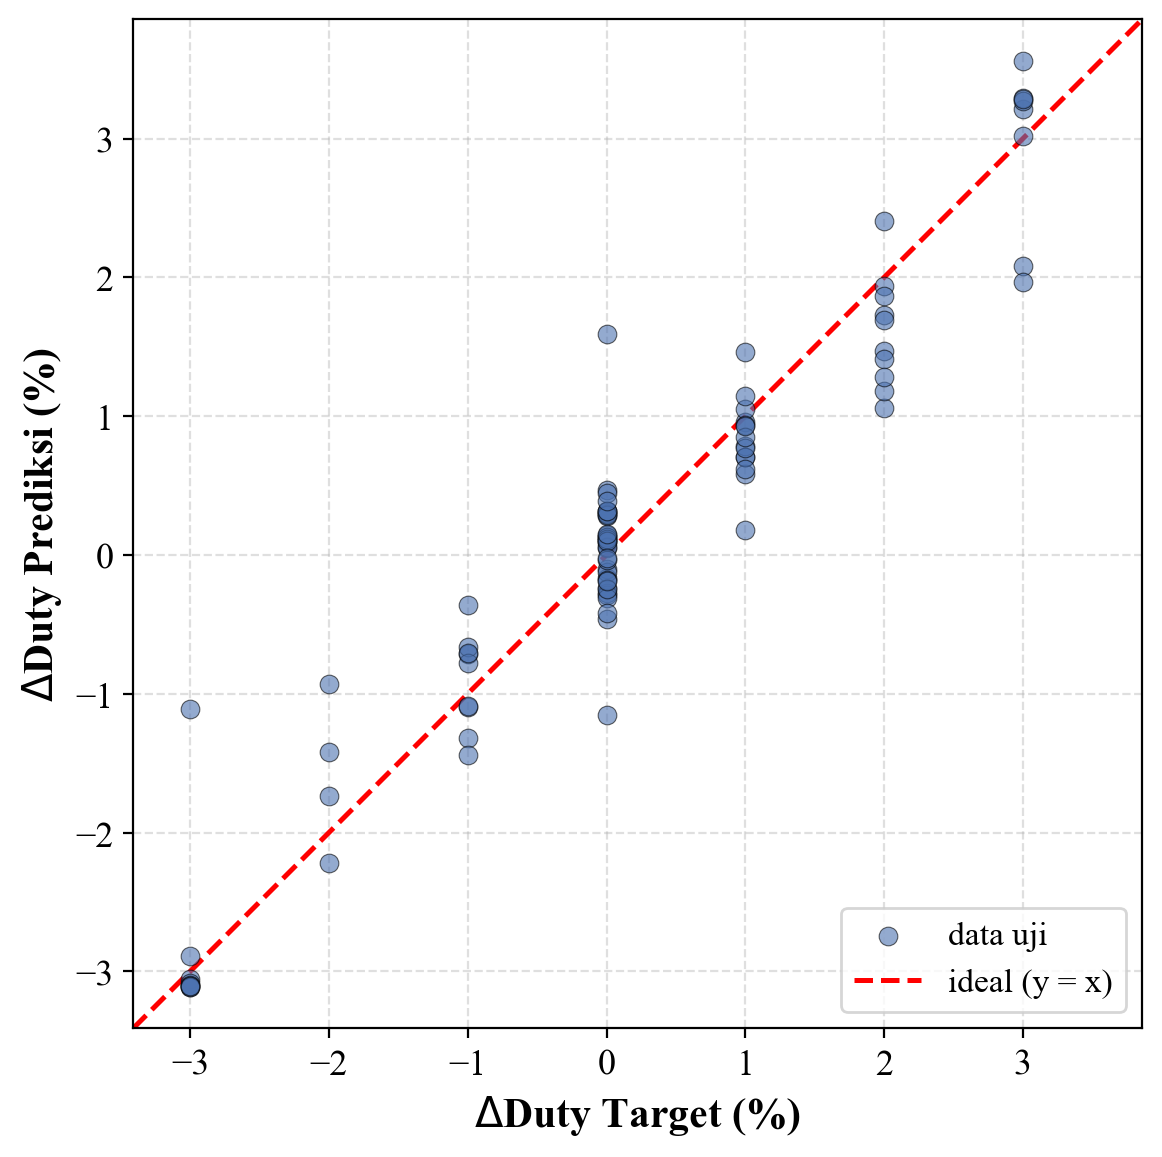
\includegraphics[width=0.75\linewidth]{gambar/target_vs_prediksi_mlp341.png}
  \caption{Perbandingan target dan prediksi $\Delta duty$ model MLP 3-4-1 pada data uji.}
  \label{fig:target-vs-prediksi-nn}
\end{figure}

Koefisien determinasi $R^2 = 0{,}915$ menunjukkan bahwa model mampu menjelaskan
sekitar 91,5\% keragaman aksi kendali pada data uji. Nilai ini dihitung dari sebaran
data terhadap garis identitas, yaitu kondisi ketika nilai prediksi sama persis
dengan nilai target, sehingga benar-benar mengukur seberapa dekat keluaran model
dengan aksi kendali sebenarnya dan bukan sekadar korelasi.
Dengan $R^2$ yang tinggi disertai MAE dan RMSE yang kecil, dapat disimpulkan bahwa
model memiliki akurasi prediksi yang baik dalam menirukan aksi kendali tekanan.

\section{Karakteristik Tekanan \emph{Open-Loop} terhadap Kondisi Keran}
\label{sec:karakteristik-openloop-keran}

Sebelum mengevaluasi sistem kendali, dilakukan pengamatan karakteristik tekanan
dalam kondisi \emph{open-loop}, yaitu \emph{duty cycle} ditetapkan secara manual
tanpa aksi kontroler ($\Delta duty = 0$). Pengamatan ini bertujuan untuk memahami
hubungan antara \emph{duty cycle}, jumlah keran yang terbuka, dan tekanan
keluaran sistem pompa. Data diambil dari fase stabil pada sesi pengambilan data
pelatihan, sehingga mencerminkan karakteristik nyata beban hidraulik.
Hasil rangkuman disajikan pada Tabel~\ref{tab:openloop-keran-duty}.

\begin{table}[H]
\centering
\caption{Tekanan \emph{open-loop} rata-rata (bar) pada berbagai kondisi keran dan \emph{duty cycle}}
\label{tab:openloop-keran-duty}
\begin{tabularx}{\linewidth}{|>{\centering\arraybackslash}X|>{\centering\arraybackslash}X|>{\centering\arraybackslash}X|>{\centering\arraybackslash}X|>{\centering\arraybackslash}X|>{\centering\arraybackslash}X|}
\hline
\textbf{\emph{Duty} (\%)} &
\textbf{0 Keran} &
\textbf{1 Keran} &
\textbf{2 Keran} &
\textbf{3 Keran} &
\textbf{4 Keran} \\
\hline
60 & 0,015 & 0,014 & 0,011 & 0,013 & 0,010 \\ \hline
70 & 0,194 & 0,098 & 0,088 & 0,079 & 0,073 \\ \hline
80 & 0,404 & 0,281 & 0,230 & 0,205 & 0,198 \\ \hline
90 & 0,571 & 0,503 & 0,411 & 0,357 & 0,308 \\ \hline
95 & 0,916 & 0,530 & 0,418 & 0,294 & 0,285 \\ \hline
\end{tabularx}
\end{table}

\begin{figure}[htbp]
\centering
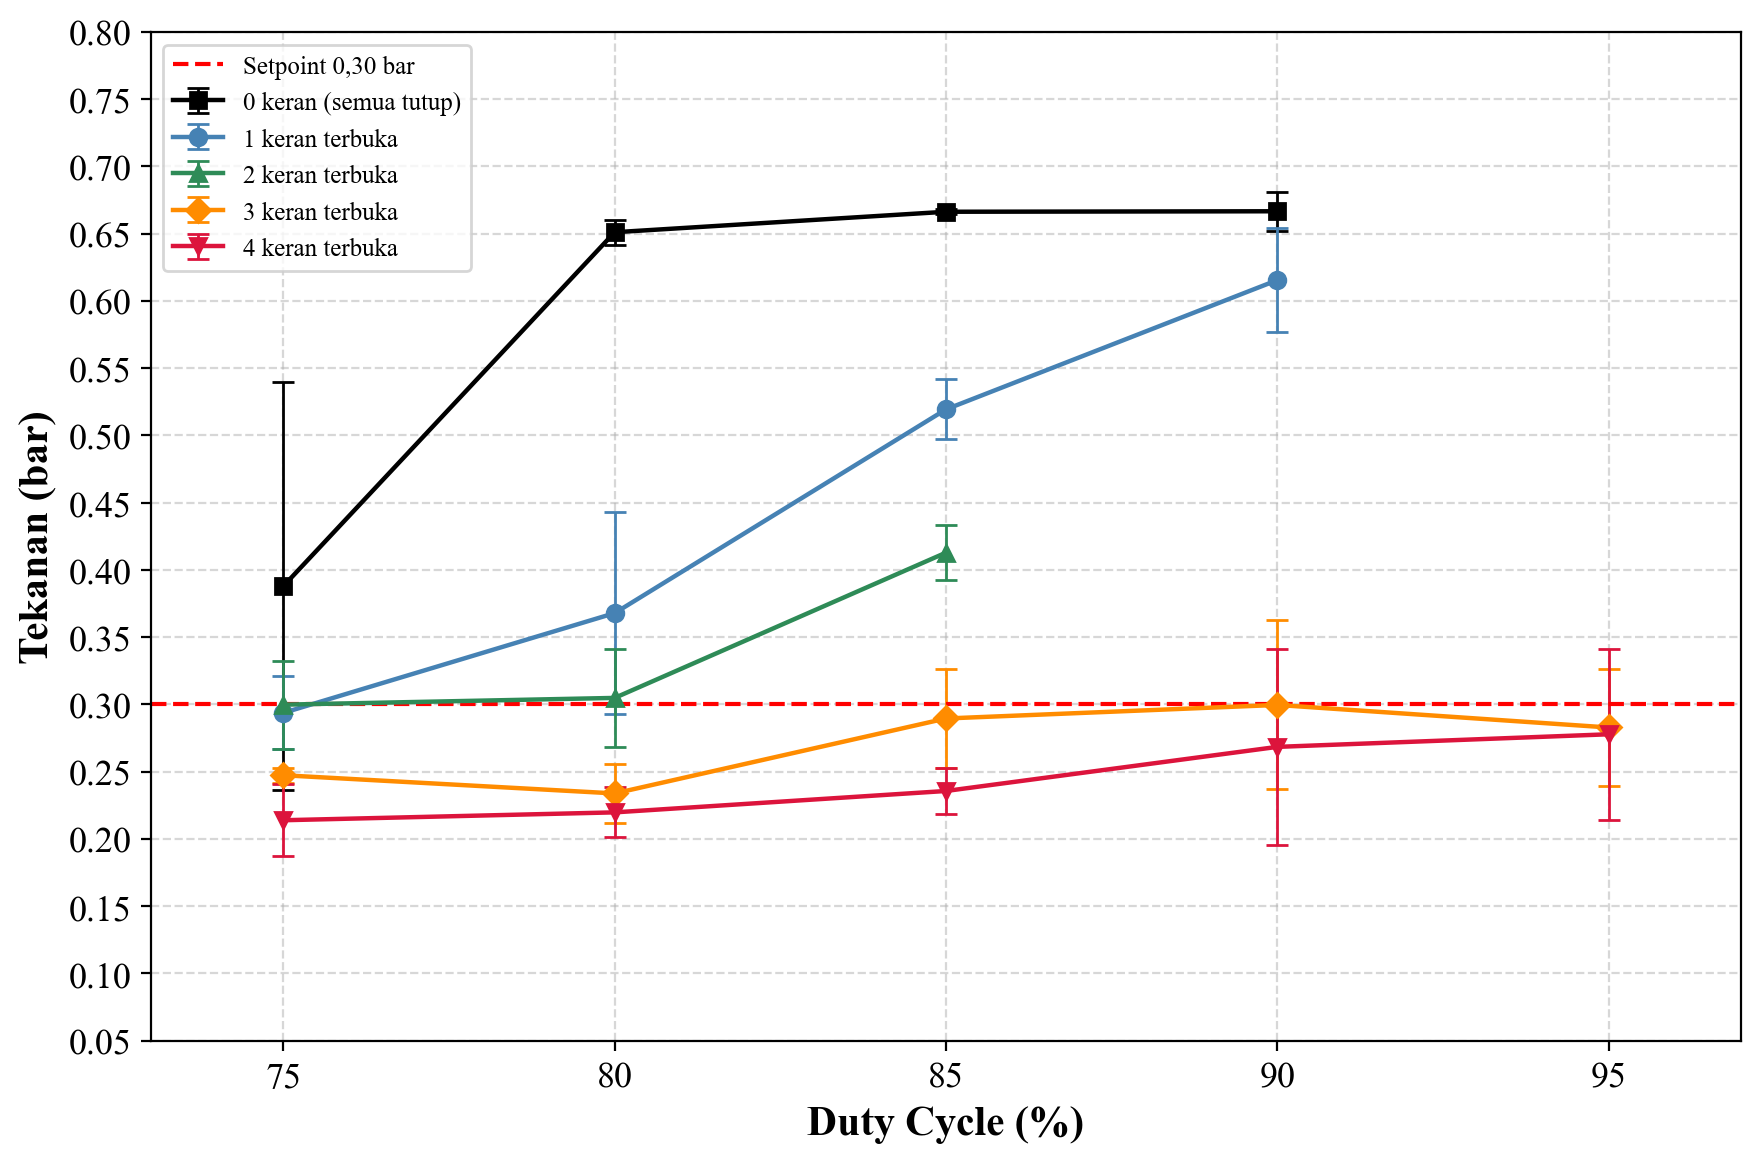
\includegraphics[width=0.82\textwidth]{gambar/grafik_openloop_keran_duty}
\caption{Karakteristik tekanan \emph{open-loop} terhadap \emph{duty cycle} pada berbagai kondisi keran}
\label{fig:grafik-openloop-keran}
\end{figure}

Tabel~\ref{tab:openloop-keran-duty} dan Gambar~\ref{fig:grafik-openloop-keran}
memperlihatkan beberapa pola penting.
Pertama, pada \emph{duty} 60\% seluruh kondisi keran menghasilkan tekanan sangat
rendah ($\approx$0,01~bar), menunjukkan bahwa pompa berada di bawah tegangan
minimum operasionalnya.
Kedua, semakin banyak keran yang terbuka, semakin rendah tekanan yang terbentuk
pada \emph{duty cycle} yang sama karena hambatan hidraulik berkurang dan debit
mengalir lebih bebas. Pola ini konsisten di seluruh rentang \emph{duty} 70--95\%.
Ketiga, dari seluruh kombinasi yang diuji, hanya kondisi 4 keran pada
\emph{duty} 90\% yang menghasilkan tekanan paling mendekati \emph{setpoint}
0,30~bar (0,308~bar), sedangkan kondisi lain membutuhkan interpolasi atau
berada jauh dari \emph{setpoint}.
Keempat, kondisi 0 keran pada \emph{duty} 95\% menghasilkan tekanan 0,916~bar,
jauh melampaui \emph{setpoint}, sehingga sistem tidak dapat beroperasi aman
tanpa membuka setidaknya satu keran.
Karakteristik ini membuktikan bahwa setiap perubahan kondisi keran membutuhkan
\emph{duty cycle} yang berbeda untuk mencapai tekanan yang sama, dan tidak ada
satu nilai \emph{duty} tunggal yang berlaku untuk semua kondisi.
Inilah yang menjadi dasar utama perlunya kendali \emph{closed-loop} berbasis
\emph{neural network}: sistem harus mampu menyesuaikan \emph{duty cycle} secara
adaptif terhadap beban hidraulik yang berubah-ubah.

\section{Pengujian Sistem Kendali Tekanan}
\label{sec:pengujian-sistem-kendali}

Pengujian sistem kendali tekanan dilakukan untuk melihat kemampuan kontroler
\emph{neural network} dalam menjaga tekanan air agar mendekati nilai
\emph{setpoint}. Pengujian dibagi menjadi tiga: (1)~penjejakan \emph{setpoint}
pada berbagai jumlah keran,
(2)~respons terhadap perubahan \emph{setpoint} (Tabel~\ref{tab:respons-setpoint}),
dan (3)~rejeksi gangguan akibat perubahan beban keran
(Tabel~\ref{tab:respons-gangguan-beban}). Pada setiap pengujian, kontroler
mengambil keputusan setiap 3~detik dan menghasilkan perubahan \emph{duty cycle}
($\Delta duty$) yang diakumulasi menjadi nilai \emph{duty cycle} aktual.
Pengujian pertama menilai kemampuan kontroler mencapai \emph{setpoint} 0,30~bar
pada tiap kondisi jumlah keran (0--4) yang merepresentasikan beban berbeda.
Hasilnya disajikan pada Tabel~\ref{tab:respons-nn-keran}.

\begin{table}[H]
\centering
\caption{Respons kontroler NN pada berbagai jumlah keran (\emph{setpoint} 0,30 bar)}
\label{tab:respons-nn-keran}
\begin{tabularx}{\linewidth}{|c|>{\centering\arraybackslash}X|>{\centering\arraybackslash}X|>{\centering\arraybackslash}X|>{\centering\arraybackslash}X|>{\centering\arraybackslash}X|>{\centering\arraybackslash}X|}
\hline
\textbf{Keran} &
\textbf{\emph{Duty} Awal (\%)} &
\textbf{\emph{Duty} Settle (\%)} &
\textbf{Tekanan Settle (bar)} &
\textbf{Error (bar)} &
\textbf{\emph{Settling Time} (s)} &
\textbf{$n$} \\
\hline
4 & 80,0 & 90,2 & 0,299 & $+$0,001 & 15,2 & 102 \\
\hline
3 & 80,0 & 80,8 & 0,293 & $+$0,007 & 0,0 & 41 \\
\hline
2 & 80,0 & 78,8 & 0,309 & $-$0,009 & 3,9 & 66 \\
\hline
1 & 78,7 & 76,4 & 0,299 & $+$0,001 & 2,7 & 49 \\
\hline
0 & 80,0 & 70,0 & 0,517 & $-$0,217 & (saturasi) & 41 \\
\hline
\end{tabularx}
\end{table}

Kontroler berhasil mencapai \emph{setpoint} 0,30~bar pada kondisi 4, 3, 2, dan 1 keran
dengan \emph{error} tunak sangat kecil ($\leq$0,009~bar). Pada 4 keran, kontroler
menaikkan \emph{duty cycle} hingga sekitar 90\% (\emph{settling} $\approx$15~detik).
Pada jumlah keran lebih sedikit, \emph{duty cycle} justru diturunkan karena tekanan
cenderung berada di atas \emph{setpoint}. Sebaliknya, pada kondisi 0 keran (seluruh
keran tertutup), tekanan tetap 0,517~bar meskipun \emph{duty cycle} telah berada pada
batas bawah 70\%, sehingga \emph{setpoint} tidak tercapai. Kondisi ini merupakan
saturasi aktuator akibat keterbatasan fisik, yaitu keluaran minimum pompa yang
melebihi \emph{setpoint} pada beban sangat tertutup, bukan kegagalan kontroler.
Dimana pada kondisi ini air terperangkap di dalam pipa dan pompa tidak dapat 
menurunkan tekanannya lebih jauh.

Untuk memperjelas cara kerja kontroler, Gambar~\ref{fig:ilustrasi-respons}
menampilkan satu contoh respons (kondisi 4 keran). Saat kontroler diaktifkan,
tekanan masih berada di bawah \emph{setpoint}, lalu kontroler menaikkan
\emph{duty cycle} secara bertahap sehingga tekanan naik dan mencapai \emph{setpoint}
0,30~bar dalam waktu sekitar 15~detik. Respons untuk seluruh kondisi jumlah keran
(0--4) ditunjukkan pada Tabel~\ref{tab:respons-nn-keran-grid}, dengan kolom
kiri menampilkan respons tekanan dan kolom kanan respons \emph{duty cycle}.

\begin{figure}[htbp]
  \centering
  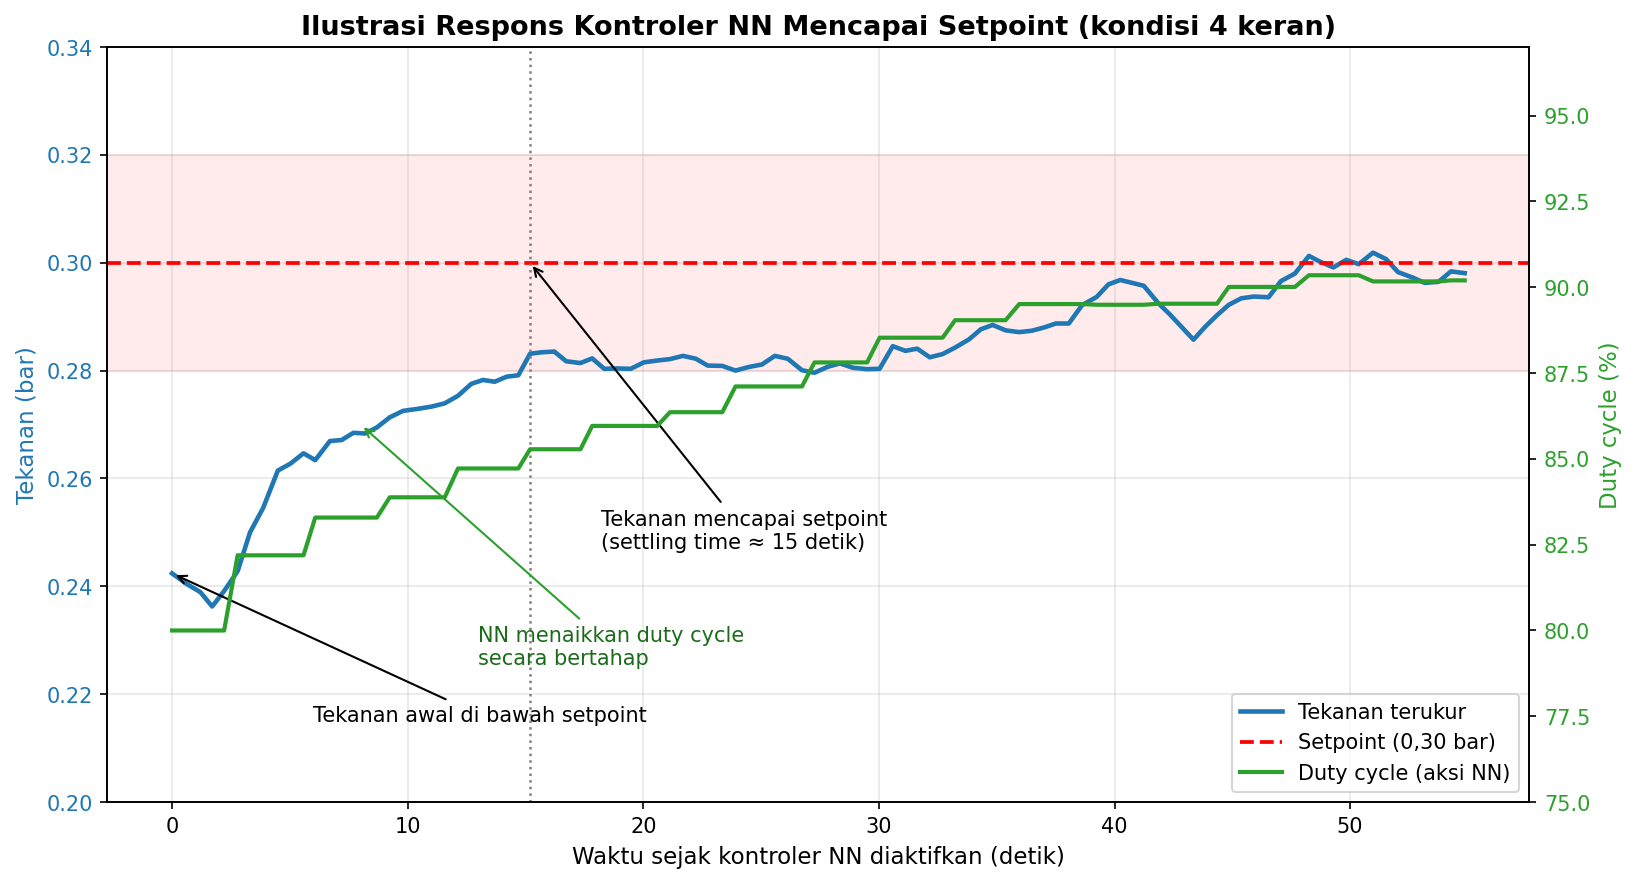
\includegraphics[width=0.92\textwidth]{gambar/ilustrasi_respons_nn}
  \caption{Ilustrasi respons kontroler NN mencapai \emph{setpoint} (kondisi 4 keran).
  Tekanan (biru) naik menuju \emph{setpoint} 0,30~bar seiring kontroler menaikkan
  \emph{duty cycle} (hijau) secara bertahap.}
  \label{fig:ilustrasi-respons}
\end{figure}

% Helper untuk menampilkan gambar respons pada sel tabel
\newcommand{\respfig}[1]{\includegraphics[width=0.40\textwidth]{gambar/#1}}

\begin{table}[H]
\centering
\caption{Respons kontroler NN menuju \emph{setpoint} 0,30~bar (keran 0--4)}
\label{tab:respons-nn-keran-grid}
\renewcommand{\arraystretch}{1.2}

\begin{tabular}{|
>{\centering\arraybackslash}m{1cm}|
>{\centering\arraybackslash}m{0.42\textwidth}|
>{\centering\arraybackslash}m{0.42\textwidth}|}
\hline
\textbf{Keran} &
\textbf{Respon Tekanan} &
\textbf{\emph{Duty Cycle}} \\
\hline

0 & \respfig{respons_tekanan_keran0} & \respfig{respons_duty_keran0} \\
\hline
1 & \respfig{respons_tekanan_keran1} & \respfig{respons_duty_keran1} \\
\hline
2 & \respfig{respons_tekanan_keran2} & \respfig{respons_duty_keran2} \\
\hline
3 & \respfig{respons_tekanan_keran3} & \respfig{respons_duty_keran3} \\
\hline
4 & \respfig{respons_tekanan_keran4} & \respfig{respons_duty_keran4} \\
\hline

\end{tabular}
\end{table}

Pengujian kedua menilai respons kontroler saat \emph{setpoint} diubah pada
beban (jumlah keran) tetap. \emph{Setpoint} divariasikan berurutan
0,25~$\rightarrow$~0,30~$\rightarrow$~0,35~$\rightarrow$~0,30~$\rightarrow$~0,25~bar
(dua kenaikan dan dua penurunan), masing-masing sebagai satu episode. Hasilnya
dirangkum pada Tabel~\ref{tab:respons-setpoint} dan profil responsnya pada
Gambar~\ref{fig:respons-setpoint}.

\begin{table}[H]
\centering
\caption{Respons sistem terhadap perubahan \emph{setpoint}}
\label{tab:respons-setpoint}
\begin{tabularx}{\linewidth}{|c|>{\centering\arraybackslash}X|>{\centering\arraybackslash}X|>{\centering\arraybackslash}X|>{\centering\arraybackslash}X|>{\centering\arraybackslash}X|}
\hline
\textbf{No.} &
\textbf{\emph{Setpoint} (bar)} &
\textbf{Tekanan Awal (bar)} &
\textbf{Tekanan Stabil (bar)} &
\textbf{\emph{Settling Time} (s)} &
\textbf{Error Stabil (bar)} \\
\hline
1 & 0,25 & 0,189 & 0,265 & 3,8 & $-$0,015 \\
\hline
2 & 0,30 & 0,216 & 0,293 & 4,2 & $+$0,007 \\
\hline
3 & 0,35 & 0,299 & 0,341 & 6,6 & $+$0,009 \\
\hline
4 & 0,30 & 0,346 & 0,308 & 4,7 & $-$0,008 \\
\hline
5 & 0,25 & 0,299 & 0,244 & 5,5 & $+$0,006 \\
\hline
\end{tabularx}
\end{table}

\begin{figure}[htbp]
  \centering
  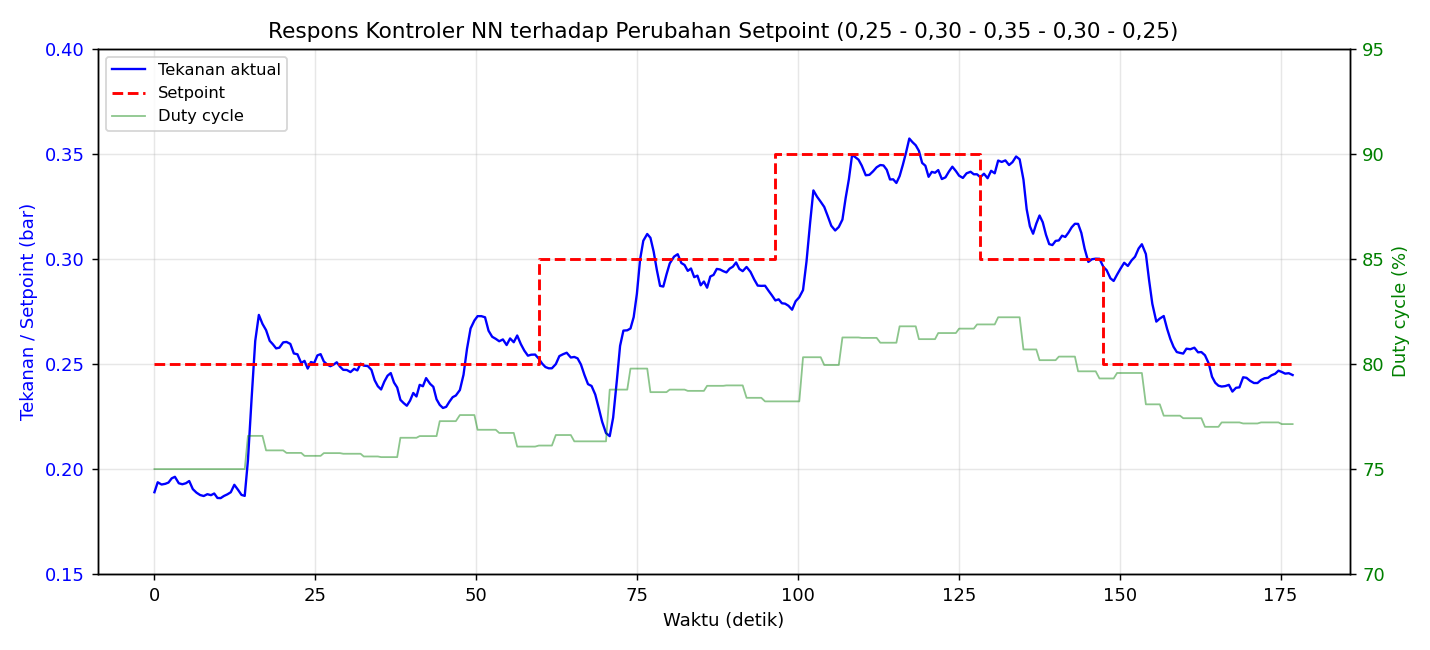
\includegraphics[width=\textwidth]{gambar/respons_setpoint_nn}
  \caption{Respons kontroler NN terhadap perubahan \emph{setpoint}
  (0,25--0,30--0,35--0,30--0,25~bar) pada beban tetap. Tekanan aktual (biru)
  mengikuti setiap perubahan \emph{setpoint} (merah), dengan \emph{duty cycle}
  (hijau) menyesuaikan secara otomatis.}
  \label{fig:respons-setpoint}
\end{figure}

Data pada tabel~\ref{tab:respons-setpoint} menunjukkan kontroler NN mampu menjejak setiap
perubahan \emph{setpoint} dengan \emph{error} tunak kecil ($\leq$0,015~bar) dan
\emph{settling time} yang singkat, yaitu berkisar 4--7~detik. Respons yang cepat
ini teramati baik saat pompa baru dinyalakan (episode~1, tekanan naik dari
0,189~bar menuju 0,25~bar) maupun saat sistem telah berjalan (episode~2--5),
serta pada perubahan dua arah, yaitu kenaikan (ke 0,30 dan 0,35~bar) dan
penurunan (kembali ke 0,30 dan 0,25~bar). Hal ini menunjukkan kontroler NN tidak
hanya bekerja pada \emph{setpoint} pelatihan utama (0,30~bar), tetapi juga mampu
menggeneralisasi ke \emph{setpoint} lain (0,25 dan 0,35~bar) dengan respons dua
arah yang stabil dan tanpa osilasi berlebih.

\begin{table}[H]
\centering
\caption{Respons sistem terhadap gangguan perubahan jumlah keran (\emph{setpoint} 0,30 bar)}
\label{tab:respons-gangguan-beban}
\begin{tabularx}{\linewidth}{|c|>{\raggedright\arraybackslash\hsize=1.5\hsize}X|>{\centering\arraybackslash\hsize=0.95\hsize}X|>{\centering\arraybackslash\hsize=0.85\hsize}X|>{\centering\arraybackslash\hsize=0.85\hsize}X|>{\centering\arraybackslash\hsize=0.85\hsize}X|}
\hline
\textbf{No.} &
\textbf{Jenis Gangguan} &
\textbf{Tekanan Sebelum (bar)} &
\textbf{Deviasi Maks (bar)} &
\textbf{Tekanan Pulih (bar)} &
\textbf{Waktu Pemulihan (s)} \\
\hline
1 & 2 $\rightarrow$ 4 keran (buka) & 0,293 & 0,092 & 0,257 & -- (saturasi) \\
\hline
2 & 4 $\rightarrow$ 2 keran (tutup) & 0,261 & 0,117 & 0,310 & 15,4 \\
\hline
3 & 2 $\rightarrow$ 3 keran (buka) & 0,293 & 0,054 & 0,283 & 13,2 \\
\hline
4 & 3 $\rightarrow$ 1 keran (tutup) & 0,293 & 0,212 & 0,309 & 9,3 \\
\hline
\end{tabularx}
\end{table}

Gangguan diberikan dengan mengubah jumlah keran secara mendadak
saat kontroler sedang menjaga tekanan pada \emph{setpoint}
0,30~bar. Membuka keran
(menambah jumlah) menyebabkan tekanan turun sehingga kontroler
menaikkan \emph{duty cycle}, sedangkan menutup keran (mengurangi
jumlah) menyebabkan tekanan naik sehingga kontroler menurunkan
\emph{duty cycle}. \emph{Deviasi maksimum} menyatakan simpangan
tekanan terbesar terhadap \emph{setpoint} akibat gangguan, dan
\emph{waktu pemulihan} adalah waktu yang dibutuhkan tekanan untuk
kembali dalam interval $\pm$0,02~bar.

Hasil menunjukkan kontroler mampu menolak gangguan dan mengembalikan tekanan ke
\emph{setpoint} pada gangguan menutup keran maupun membuka keran. Pada gangguan
terbesar (3~$\rightarrow$~1 keran) tekanan sempat melonjak hingga deviasi 0,212~bar,
namun kontroler memulihkannya ke 0,30~bar dalam 9,3~detik. Pengecualian terjadi pada
gangguan 2~$\rightarrow$~4 keran: tekanan turun dan kontroler menaikkan \emph{duty
cycle} hingga batas 95\%, tetapi tekanan hanya pulih ke 0,257~bar (tidak kembali ke
\emph{setpoint}). Hal ini konsisten dengan hasil Tabel~\ref{tab:respons-nn-keran},
yaitu pada 4 keran terbuka pompa berada pada batas kemampuannya (saturasi aktuator).
Secara umum, semakin besar gangguan, semakin besar deviasi tekanannya, namun selama
\emph{setpoint} masih berada dalam rentang kemampuan pompa, kontroler berhasil
memulihkan tekanan tanpa osilasi berlebih. Profil respons gangguan ditunjukkan pada
Gambar~\ref{fig:respons-gangguan}.

Jika dibandingkan dengan kontroler PID yang digunakan pada penelitian
sebelumnya~\parencite{anakits,anakub}, kontroler NN yang diusulkan memiliki
waktu pemulihan yang lebih lambat. Pada penelitian terdahulu, kontroler PID
mampu memulihkan tekanan dalam waktu 3--6~detik, sedangkan kontroler NN pada
penelitian ini memerlukan 9,3--15,4~detik tergantung besarnya gangguan.
Perbedaan ini disebabkan oleh sifat kontroler NN yang berbasis data —
\emph{forward pass} MLP hanya menghasilkan $\Delta duty$ terbatas per langkah
dan memerlukan beberapa siklus untuk mengoreksi kesalahan besar. Meskipun
demikian, kontroler NN memiliki kelebihan dalam menghasilkan respons yang
lebih halus tanpa osilasi berlebih dan mampu meniru perilaku operator secara
langsung tanpa pemodelan matematis \emph{plant} secara eksplisit. Untuk
penelitian selanjutnya, disarankan peningkatan respons kontroler NN agar
waktu pemulihan dapat mendekati atau melampaui kinerja PID, misalnya dengan
menambahkan aksi integral pada struktur kendali atau mengombinasikan NN dengan
kontroler konvensional (\emph{hybrid control}).

\begin{figure}[H]
  \centering
  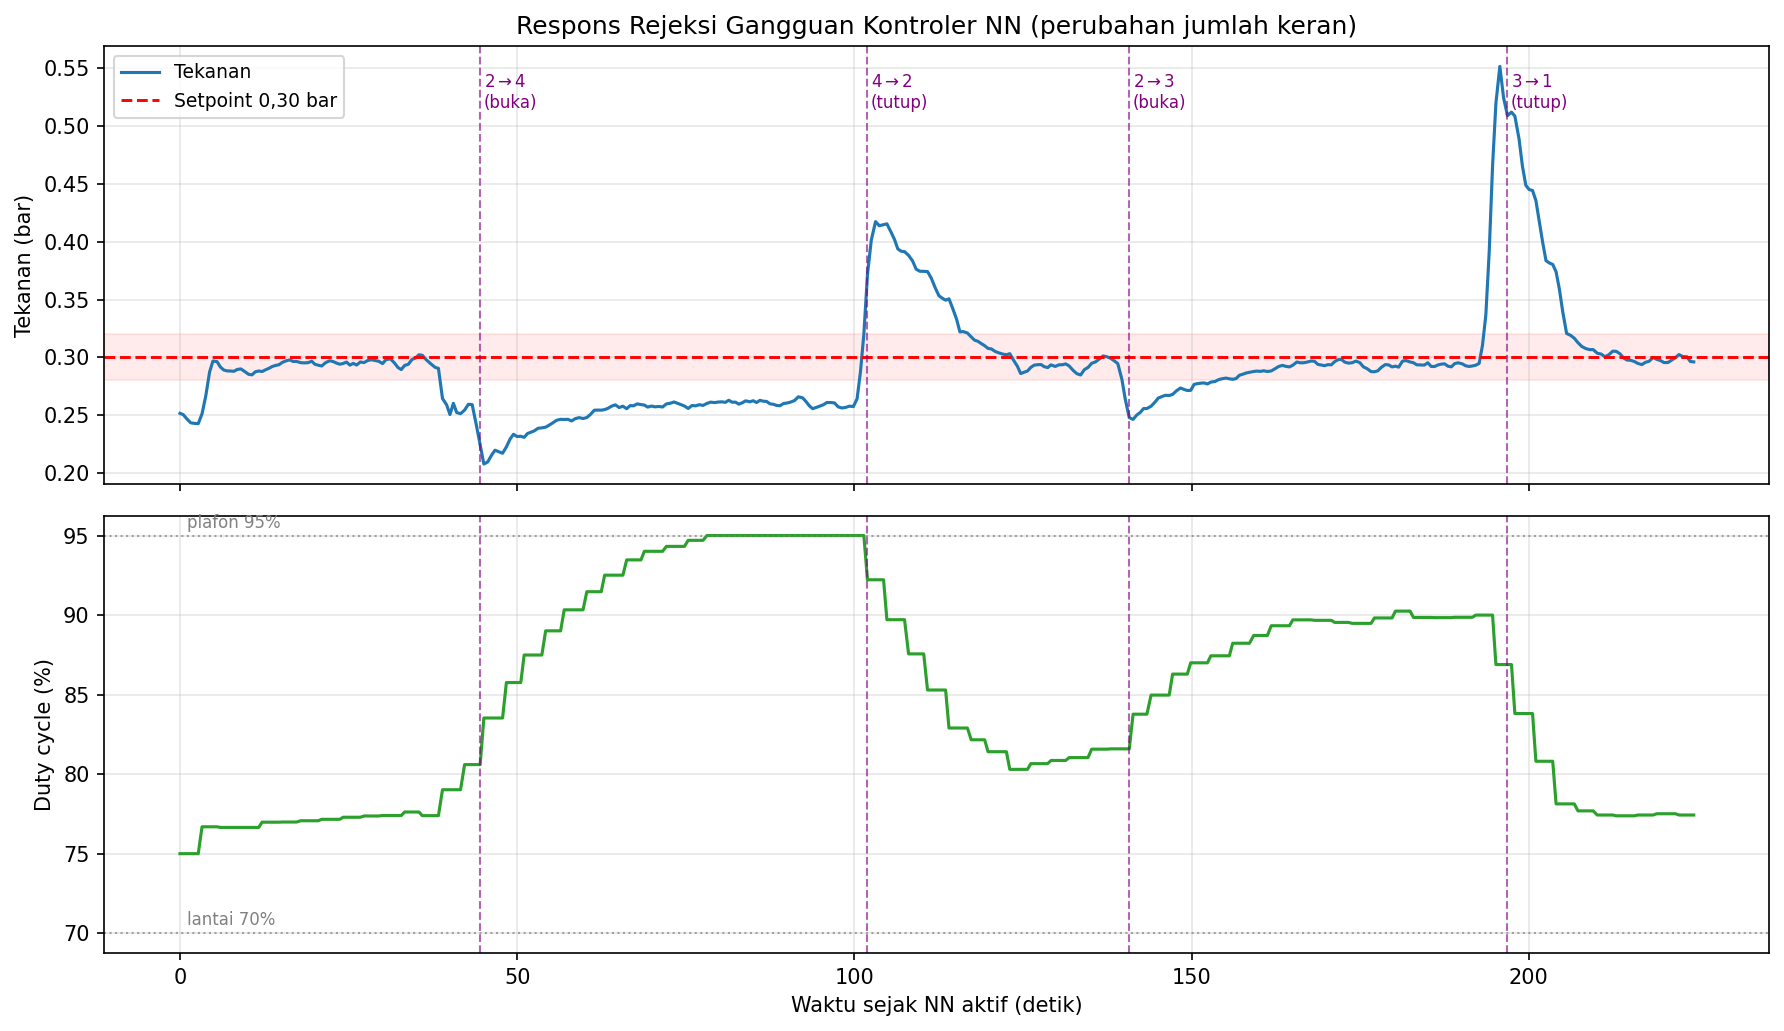
\includegraphics[width=\textwidth]{gambar/respons_gangguan_nn}
  \caption{Respons rejeksi gangguan kontroler NN terhadap perubahan jumlah keran
  secara mendadak (\emph{setpoint} 0,30 bar). Garis putus-putus menandai saat gangguan;
  panel atas tekanan, panel bawah \emph{duty cycle}.}
  \label{fig:respons-gangguan}
\end{figure}

\section{Pengujian Debit Air}
\label{sec:pengujian-debit}

Pengujian debit air dilakukan untuk mengetahui laju aliran (\emph{flow rate})
yang disalurkan sistem pada berbagai kondisi beban keran, sekaligus menampilkan
komparasi antara kondisi dengan kendali \emph{neural network} (NN) dan kondisi
\emph{open-loop} dengan \emph{duty cycle} tetap. Debit diukur secara volumetrik
menggunakan empat botol penampung berkapasitas 1500~mL. Air yang keluar dari tiap
keran ditampung selama selang waktu tertentu, kemudian volume yang terkumpul
diukur menggunakan gelas ukur. Debit tiap keran dihitung dengan $Q = V/t$ dan
debit total merupakan penjumlahan debit seluruh keran yang terbuka. Seluruh
pengukuran diambil setelah aliran mencapai kondisi tunak.
Hasil pengukuran debit air dengan kendali \emph{neural network} ditunjukkan pada Tabel~\ref{tab:debit-nn}.

\begin{table}[H]
\centering
\caption{Hasil pengukuran debit air dengan kendali \emph{neural network} (mL/s)}
\label{tab:debit-nn}
\begin{tabularx}{\linewidth}{|c|>{\centering\arraybackslash}X|>{\centering\arraybackslash}X|>{\centering\arraybackslash}X|>{\centering\arraybackslash}X|>{\centering\arraybackslash}X|}
\hline
\textbf{Jumlah Keran} &
\textbf{Keran 1} &
\textbf{Keran 2} &
\textbf{Keran 3} &
\textbf{Keran 4} &
\textbf{Debit Total} \\
\hline
1 & 94,14 & -- & -- & -- & 94,14 \\
\hline
2 & 46,11 & 57,32 & -- & -- & 103,43 \\
\hline
3 & 49,13 & 61,27 & 105,33 & -- & 215,73 \\
\hline
4 & 59,33 & 60,80 & 99,33 & 59,33 & 278,80 \\
\hline
\end{tabularx}
\end{table}

\newpage
Sebagai pembanding, pengukuran diulang pada kondisi \emph{open-loop} dengan
\emph{duty cycle} dipatok tetap 90\% tanpa kendali NN, menggunakan selang waktu
penampungan tetap $t = 15$~detik. Hasilnya disajikan pada
Tabel~\ref{tab:debit-openloop}, lengkap dengan tekanan yang terukur pada tiap
kondisi.

\begin{table}[H]
\centering
\caption{Hasil pengukuran debit air \emph{open-loop} \emph{duty} 90\% (mL/s)}
\label{tab:debit-openloop}
\begin{tabularx}{\linewidth}{|c|>{\centering\arraybackslash}X|>{\centering\arraybackslash}X|>{\centering\arraybackslash}X|>{\centering\arraybackslash}X|>{\centering\arraybackslash}X|>{\centering\arraybackslash}X|}
\hline
\textbf{Jumlah Keran} &
\textbf{Keran 1} &
\textbf{Keran 2} &
\textbf{Keran 3} &
\textbf{Keran 4} &
\textbf{Debit Total} &
\textbf{Tekanan (bar)} \\
\hline
1 & 64,67 & -- & -- & -- & 64,67 & 0,661 \\
\hline
2 & 57,33 & 26,00 & -- & -- & 83,33 & 0,626 \\
\hline
3 & 56,93 & 23,60 & 113,33 & -- & 193,87 & 0,701 \\
\hline
4 & 57,33 & 23,60 & 113,67 & 31,53 & 226,13 & 0,650 \\
\hline
\end{tabularx}
\end{table}

Sebagai komparasi, rekapitulasi debit total pada kedua kondisi disajikan pada
Tabel~\ref{tab:debit-rekap}, dinyatakan dalam satuan mL/s dan L/menit. Tabel ini
ditampilkan sebagai pembanding data, bukan sebagai penilaian keunggulan salah
satu kondisi, karena keduanya berada pada titik kerja yang berbeda.

\begin{table}[H]
\centering
\caption{Rekapitulasi debit total pada kondisi kendali NN dan \emph{open-loop} \emph{duty} 90\%}
\label{tab:debit-rekap}
\begin{tabularx}{\linewidth}{|c|>{\centering\arraybackslash}X|>{\centering\arraybackslash}X|>{\centering\arraybackslash}X|>{\centering\arraybackslash}X|}
\hline
\textbf{Jumlah Keran} &
\textbf{NN (mL/s)} &
\textbf{NN (L/mnt)} &
\textbf{\emph{Open-Loop} (mL/s)} &
\textbf{\emph{Open-Loop} (L/mnt)} \\
\hline
1 & 94,14  & 5,65  & 64,67  & 3,88  \\
\hline
2 & 103,43 & 6,21  & 83,33  & 5,00  \\
\hline
3 & 215,73 & 12,94 & 193,87 & 11,63 \\
\hline
4 & 278,80 & 16,73 & 226,13 & 13,57 \\
\hline
\end{tabularx}
\end{table}

Hasil pengukuran menunjukkan debit total meningkat seiring bertambahnya jumlah
keran yang terbuka, baik pada kondisi kendali NN maupun \emph{open-loop}. Pada
kondisi kendali NN debit total naik dari 94,14~mL/s (5,65~L/menit) saat satu
keran menjadi 278,80~mL/s (16,73~L/menit) saat empat keran, sedangkan pada
kondisi \emph{open-loop} naik dari 64,67~mL/s (3,88~L/menit) menjadi
226,13~mL/s (13,57~L/menit). Peningkatan ini sesuai dengan prinsip bahwa
penambahan jalur keluaran memperbesar laju aliran total sistem.

Kedua kondisi pada Tabel~\ref{tab:debit-rekap} berada pada titik kerja yang
berbeda. Pada kondisi kendali NN tekanan diregulasi pada \emph{setpoint}
0,30~bar, sedangkan pada kondisi \emph{open-loop} nilai \emph{duty} dipatok tetap
90\%. Selain itu, derajat bukaan tiap keran dalam pengujian ini mengikuti
konvensi yang ditetapkan, yaitu satu keran terbuka setara dengan setengah bukaan
penuh, sehingga laju aliran tiap keran memang berbeda-beda sesuai derajat
bukaannya. Oleh karena itu, kedua tabel berfungsi sebagai karakterisasi debit
pada masing-masing kondisi, dan ditampilkan berdampingan semata-mata sebagai
komparasi data.

